\documentclass[11pt]{article}

\usepackage{fancybox}



\usepackage{color}
\usepackage{url}
\usepackage[margin=1in]{geometry}


\renewcommand{\textfraction}{0.0}
\renewcommand{\topfraction}{1.0}
%\renewcommand{\textfloatsep}{5mm}


\usepackage{comment}
% Definitions of handy macros can go here
\usepackage{amsmath,amssymb,amsthm,bm,mathtools}
\usepackage{multirow}
\usepackage{natbib}
%\usepackage{dsfont,multirow,hyperref,setspace,natbib,enumerate}
\usepackage{dsfont,multirow,hyperref,setspace,enumerate}
\hypersetup{colorlinks,linkcolor={blue},citecolor={blue},urlcolor={red}}
\usepackage{algpseudocode,algorithm}
\algnewcommand\algorithmicinput{\textbf{Input:}}
\algnewcommand\algorithmicoutput{\textbf{Output:}}
\algnewcommand\INPUT{\item[\algorithmicinput]}
\algnewcommand\OUTPUT{\item[\algorithmicoutput]}

\mathtoolsset{showonlyrefs=true}



\theoremstyle{plain}
\newtheorem{thm}{Theorem}[section]
\newtheorem{lem}{Lemma}
\newtheorem{prop}{Proposition}
\newtheorem{pro}{Property}
\newtheorem{assumption}{Assumption}

\theoremstyle{definition}
\newtheorem{defn}{Definition}
\newtheorem{cor}{Corollary}
\newtheorem{example}{Example}
\newtheorem{rmk}{Remark}


\renewcommand{\thefigure}{{S\arabic{figure}}}%
\renewcommand{\thetable}{{S\arabic{table}}}%
\renewcommand{\figurename}{{Supplementary Figure}}
\renewcommand{\tablename}{{Supplementary Table}}
\setcounter{figure}{0}
\setcounter{table}{0}


\def\MLET{\hat \Theta_{\text{MLE}}}
\newcommand{\cmt}[1]{{\leavevmode\color{red}{#1}}}



\usepackage{dsfont}

\usepackage{multirow}

\DeclareMathOperator*{\minimize}{minimize}

\usepackage{wrapfig}

\usepackage{mathtools}
\mathtoolsset{showonlyrefs}
\newcommand*{\KeepStyleUnderBrace}[1]{%f
  \mathop{%
    \mathchoice
    {\underbrace{\displaystyle#1}}%
    {\underbrace{\textstyle#1}}%
    {\underbrace{\scriptstyle#1}}%
    {\underbrace{\scriptscriptstyle#1}}%
  }\limits
}
\usepackage{xr}
\externaldocument{ordinalTv3}
\input macros.tex
\setlength\parindent{0pt}
\allowdisplaybreaks



\title{Supplements for ``Tensor denoising and completion based on ordinal observations''}


%\author{%
%Chanwoo Lee \\
%University of Wisconsin -- Madison\\
 %\texttt{chanwoo.lee@wisc.edu} \\
%\And
%Miaoyan Wang \\
%University of Wisconsin -- Madison\\
%\texttt{miaoyan.wang@wisc.edu} \\
%}

\begin{document}


\begin{center}
\begin{spacing}{1.5}
\textbf{\Large Supplements for ``Tensor denoising and completion based on ordinal observations''}
\end{spacing}
\end{center}

\section{Proofs}
\subsection{Estimation error for tensor denoising}
\begin{proof}[Proof of Theorem~\ref{thm:rate}]
We suppress the subscript $\Omega$ in the proof, because the tensor denoising assumes complete observation $\Omega=[d_1]\times \cdots \times [d_K]$. It follows from the expression of $\flogl(\Theta)$ that
\begin{align}\label{eq:property}
{\partial \flogl\over \partial \theta_\omega}&=\sum_{\ell\in[L]}\mathds{1}_{\{y_{\omega}=\ell\}}
{\dot{g}_\ell(\theta_\omega)\over g_\ell(\theta_\omega)},\notag\\
{\partial^2 \flogl\over \partial \theta_\omega^2}&=\sum_{\ell\in[L]}\mathds{1}_{\{y_\omega=\ell\}}{\ddot{g}_\ell(\theta_\omega)g_\ell(\theta_\omega)-\dot{g}^2_\ell(\theta_\omega)\over g^2_\ell(\theta_\omega)}\ \text{and}\quad
{\partial^2 \flogl\over \partial \theta_\omega \theta_\omega'}=0\ \text{if}\ \omega\neq \omega',
\end{align}
for all $\omega\in[d_1]\times \cdots \times [d_K]$.
Define $d_{\text{total}}=\prod_k d_k$. Let $\fplogl\in\mathbb{R}^{d_1\times\cdots\times d_K}$ denote the tensor of gradient with respect to $\Theta\in\mathbb{R}^{d_1\times \cdots\times d_K}$, and $\fpplogl$ the corresponding Hession matrix of size $d_\text{total}$-by-$d_{\text{total}}$. Here, $\Vec(\cdot)$ denotes the operation that turns a tensor into a vector. By~\eqref{eq:property}, $\fpplogl$ is a diagonal matrix. Recall that
\begin{equation}\label{eq:bound}
U_\alpha=\max_{\ell\in[L],|\theta|\leq \alpha}{|\dot{g}_\ell(\theta)|\over g_\ell(\theta)}>0 \quad \text{and}\quad
L_\alpha=\min_{\ell\in[L],|\theta|\leq \alpha} {\dot{g}^2_\ell(\theta)-\ddot{g}_\ell(\theta)g_\ell(\theta)\over g^2_\ell(\theta)}>0.
\end{equation}
Therefore, the entries in $\fplogl$ are upper bounded in magnitude by $U_\alpha>0$, and all diagonal entries in $\fpplogl$ are upper bounded by $-L_{\alpha}<0$.

By the second-order Taylor's expansion of $\flogl(\Theta)$ around $\trueT$, we obtain
\begin{equation}\label{eq:taylor}
\flogl(\Theta)=\flogl(\trueT)+\langle\Vec(\fplogl),\ \Vec(\Theta-\trueT)\rangle+{1\over 2}\Vec(\Theta-\trueT)^T\fpplogl(\check\Theta)\Vec(\Theta-\trueT),
\end{equation}
$\check\Theta=\gamma\trueT+(1-\gamma)\Theta$ for some $\gamma\in[0,1]$, and $\fpplogl(\check\Theta)$ denotes the $\prod_kd_k$-by-$\prod_k d_k$ Hession matrix evaluated at $\check\Theta$.

We first bound the linear term in~\eqref{eq:taylor}. Note that, by Lemma~\ref{lem:inq},
\begin{equation}\label{eq:linear}
|\langle\Vec(\fplogl(\trueT), \Vec(\Theta-\trueT)  \rangle|\leq \snormSize{}{\fplogl(\trueT)} \nnormSize{}{\Theta-\trueT},
\end{equation}
where $\snormSize{}{\cdot}$ denotes the tensor spectral norm and $\nnormSize{}{\cdot}$ denotes the tensor nuclear norm. Define
\[
s_\omega={\partial \tL_\tY\over \partial \theta_\omega}\Big|_{\Theta=\trueT} \;\; \textrm{ for all } \; \omega\in[d_1]\times\cdots\times [d_K].
\]
Based on~\eqref{eq:property} and the definition of $U_\alpha$, $\fplogl(\trueT)=\entry{s_{\omega}}$ is a random tensor whose entries are independently distributed satisfying
\begin{equation}\label{eq:norm}
\mathbb{E}(s_\omega)=0,\quad |s_\omega|\leq U_\alpha, \quad \text{for all }\omega\in[d_1]\times \cdots \times [d_K].
\end{equation}
By lemma~\ref{lem:noisytensor}, with probability at least $1-\exp(-C_1 \sum_kd_k)$, we have
\begin{equation}\label{eq:normrandom}
\snormSize{}{\fplogl(\trueT)} \leq C_2 U_\alpha\sqrt{\sum_k d_k},
\end{equation}
where $C_1, C_2$ are two positive constants that depend only on $K$. Furthermore, note that $\text{rank}(\Theta)\leq \mr$, $\text{rank}(\trueT)\leq \mr$, so $\text{rank}(\Theta-\trueT)\leq 2\mr$. By lemma~\ref{lem:nuclear}, $\nnormSize{}{\Theta-\trueT}\leq (2r_{\max})^{K-1\over 2}\FnormSize{}{\Theta-\trueT}$. Combining~\eqref{eq:linear}, \eqref{eq:norm} and \eqref{eq:normrandom}, we have that, with probability at least $1-\exp(-C_1 \sum_kd_k)$,
\begin{equation}\label{eq:linearconclusion}
|\langle \Vec(\fplogl(\trueT)), \Vec(\Theta-\trueT)  \rangle | \leq C_2 U_\alpha  \sqrt{r_{\max}^{K-1} \sum_k d_k}  \FnormSize{}{\Theta-\trueT}.
\end{equation}

We next bound the quadratic term in \eqref{eq:taylor}. Note that
\begin{align}\label{eq:quadratic}
 \Vec(\Theta-\trueT)^T \fpplogl(\check{\Theta})\Vec(\Theta-\trueT)&=\sum_\omega \left( {\partial^2\tL_{\tY}\over \partial \theta^2_\omega} \Big|_{\Theta=\check\Theta} \right)(\theta_\omega-\theta_{{\text{true}},\omega})^2 \nonumber \\
&\leq - L_\alpha\sum_{\omega}(\Theta_{\omega}-\Theta_{\text{true},\omega})^2 \nonumber \\
&=-L_\alpha\FnormSize{}{\Theta-\trueT}^2,
\end{align}
where the second line comes from the fact that  $\mnormSize{}{\check\Theta}\leq \alpha$ and the definition of $L_\alpha$.

Combining~\eqref{eq:taylor}, \eqref{eq:linearconclusion} and~\eqref{eq:quadratic}, we have that, for all $\Theta\in\tP$, with probability at least $1-\exp(-C_1 \sum_kd_k)$,
\[
\tL_\tY(\Theta)\leq \tL_{\tY}(\trueT)+C_2U_\alpha  \left(r_{\max}^{K-1}\sum_k d_k\right)^{1/2}  \FnormSize{}{\Theta-\trueT}-{L_\alpha\over 2}\FnormSize{}{\Theta-\trueT}^2.
\]
In particular, the above inequality also holds for $\hat \Theta\in\tP$. Therefore,
\[
\tL_\tY(\hat \Theta)\leq \tL_{\tY}(\trueT)+C_2U_\alpha \left(r_{\max}^{K-1}\sum_k d_k\right)^{1/2}  \FnormSize{}{\hat \Theta-\trueT}-{L_\alpha\over 2} \FnormSize{}{\hat \Theta-\trueT}^2.
\]
Since $\hat \Theta=\arg\max_{\Theta\in\tP}\tL_\tY(\Theta)$, $\tL_\tY(\hat \Theta)-\tL_{\tY}(\trueT)\geq 0$, which gives
\[
C_2U_\alpha \left(r_{\max}^{K-1}\sum_k d_k\right)^{1/2}  \FnormSize{}{\hat \Theta-\trueT}-{L_\alpha\over 2}\FnormSize{}{\hat \Theta-\trueT}^2\geq 0.
\]
Henceforth,
\[
{1\over \sqrt{\prod_k d_k}} \FnormSize{}{\hat \Theta-\trueT}\leq {2C_2U_\alpha \sqrt{r_{\max}^{K-1}\sum_k d_k}\over L_\alpha \sqrt{\prod_k d_k}}={2C_2U_\alpha r_{\max}^{(K-1)/2}\over L_\alpha} \sqrt{ \sum_k d_k \over \prod_k d_k}.
\]
This completes the proof.
\end{proof}

\begin{proof}[Proof of Corollary~\ref{cor:prediction}]
The result follows immediately from Theorem~\ref{thm:rate} and Lemma~\ref{lem:KL}.
\end{proof}

\begin{proof}[Proof of Theorem~\ref{thm:minimax}]

Let $d_{\text{total}}=\prod_{k\in[K]}d_k$, and $\gamma\in[0,1]$ be a constant to be specified later.  Our strategy is to construct a finite set of tensors $\tX=\{\Theta_i\colon i=1,\ldots \}\subset \tP$ satisfying the properties of (i)-(iv) in Lemma~\ref{lem:construction}. By Lemma~\ref{lem:construction}, such a subset of tensors exist. For any tensor  $\Theta\in\tX$, let $\mathbb{P}_{\Theta}$ denote the distribution of $\tY|\Theta$, where $\tY$ is the ordinal tensor. In particular, $\mathbb{P}_{\mathbf{0}}$ is the distribution of $\tY$ induced by the zero parameter tensor $\mathbf{0}$, i.e., the distribution of $\tY$ conditional on the parameter tensor $\Theta=\mathbf{0}$. Based on the Remark for Lemma~\ref{lem:KL}, we have
\begin{equation}\label{eq:KLbound1}
KL(\mathbb{P}_{\Theta}|| \mathbb{P}_{\mathbf{0}})\leq C \FnormSize{}{\Theta}^2,
\end{equation}
where $C={(4L-6) \dot{f}^2(0)\over  A_\alpha}>0$ is a constant independent of the tensor dimension and rank.
Combining the inequality~\eqref{eq:KLbound1} with property (iii) of $\tX$, we have
\begin{equation}\label{eq:KLbound}
\text{KL}(\mathbb{P}_{\Theta}||\mathbb{P}_{\mathbf{0}})\leq \gamma^2 R_{\max} d_{\max}.
\end{equation}
From~\eqref{eq:KLbound} and the property (i), we deduce that the condition
\begin{equation}\label{eq:totalKL}
{1\over \text{Card}(\tX)-1}\sum_{\Theta \in\tX}\text{KL}(\mathbb{P}_{\Theta}, \mathbb{P}_{\mathbf{0}})\leq \varepsilon \log_2\left\{\text{Card}(\tX)-1 \right\}
\end{equation}
holds for any $ \varepsilon \geq 0$ when $\gamma\in[0,1]$ is chosen to be sufficiently small depending on $\varepsilon$, e.g., $\gamma \leq \sqrt{3\varepsilon}$. By applying Lemma~\ref{lem:Tsybakov} to~\eqref{eq:totalKL}, and in view of the property (iv), we obtain that
\begin{equation}\label{eq:final}
\inf_{\hat \Theta}\sup_{\trueT\in \tX}\mathbb{P}\left(\FnormSize{}{\hat \Theta- \trueT}\geq  {\gamma\over 8} \min\left\{ \alpha\sqrt{d_{\text{total}}}, C^{-1/2}\sqrt{ R_{\max}d_{\max}}\right\} \right)\geq {1\over 2}\left(1-2\varepsilon-\sqrt{16 \varepsilon \over R_{\max}d_{\max}}\right).
\end{equation}
Note that $\text{Loss}(\hat \Theta, \trueT)=\FnormSize{}{\hat \Theta- \trueT}^2/d_{\text{total}}$ and $\tX\subset \tP$. By taking $\varepsilon=1/8$ and $\gamma=1/2$, we conclude from~\eqref{eq:final} that
\begin{equation}\label{eq:prob}
\inf_{\hat \Theta}\sup_{\trueT\in \tP}\mathbb{P}\left(\text{Loss}(\hat \Theta, \trueT)\geq {1 \over 256}\min\left \{ \alpha^2,  {C^{-1}R_{\max}d_{\max}\over d_{\text{total}}}\right \}\right)\geq {1\over 2}\left({3\over 4}- {2\over R_{\max}d_{\max}} \right)\geq {1\over 8}.
\end{equation}
This completes the proof.
\end{proof}

\subsection{Sample complexity for tensor completion}

\begin{proof}[Proof of Theorem~\ref{thm:completion}]

For notational convenience, we use $\MFnormSize{}{\Theta}=\sum_{\omega\in\Omega}\Theta^2_\omega$ to denote the sum of squared entries over the observed set $\Omega$, for a tensor $\Theta\in\mathbb{R}^{d_1\times \cdots \times d_K}$.

Following a similar argument as in the proof of Theorem~\ref{thm:rate}, we have
\begin{equation}\label{eq:Taylor2}
\logl(\Theta)=\logl(\trueT)+\langle\Vec(\plogl),\ \Vec(\Theta-\trueT)\rangle+{1\over 2}\Vec(\Theta-\trueT)^T\pplogl(\check\Theta)\Vec(\Theta-\trueT),
\end{equation}
where
\begin{enumerate}
\item $\plogl$ is a $d_1\times\cdots\times d_K$ tensor with $|\Omega|$ nonzero entries, and each entry is upper bounded by $U_\alpha>0$.
\item $\pplogl$ is a diagonal matrix of size $d_{\text{total}}$-by-$d_{\text{total}}$ with $|\Omega|$ nonzero entries, and each entry is upper bounded by $-L_{\alpha}<0$.
\end{enumerate}

Similar to~\eqref{eq:linear} and~\eqref{eq:quadratic}, we have
\begin{equation}\label{eq:linear2}
|\langle\Vec(\plogl),\ \Vec(\Theta-\trueT)\rangle|\leq C_2U_\alpha \sqrt{r_{\max}^{K-1}\sum_k d_k}\MFnormSize{}{\Theta-\trueT}
\end{equation}
and
\begin{equation}\label{eq:quadratic2}
\Vec(\Theta-\trueT)^T\fpplogl(\check\Theta)\Vec(\Theta-\trueT)\leq -L_\alpha \MFnormSize{}{\Theta-\trueT}^2.
\end{equation}

Combining~\eqref{eq:Taylor2}-\eqref{eq:quadratic2} with the fact that $\logl(\hat \Theta)\geq \logl(\trueT)$, we have
\begin{equation}\label{eq:sample}
\MFnormSize{}{\hat \Theta-\trueT}\leq {2C_2U_\alpha  r_{\max}^{(K-1)/2} \over L_\alpha} \sqrt{\sum_kd_k}.
\end{equation}
Lastly, we invoke the result regarding the closeness of $\Theta$ to its sampled version $\Theta_{\Omega}$, under the entrywise bound condition. Note that $\mnormSize{}{\hat\Theta-\trueT}\leq 2\alpha$ and $\text{rank}(\hat \Theta-\trueT)\leq 2\mr$. By Lemma~\ref{lem:Mnormbound}, $\anormSize{}{\hat \Theta-\trueT}\leq 2^{(3K-1)/2} \alpha \left({\prod r_k \over r_{\max}}\right)^{3/2}$. Therefore, the condition in Lemma~\ref{lem:convexity} holds with $\beta=2^{(3K-1)/2}\alpha \left({\prod r_k \over r_{\max}}\right)^{3/2}$.
Applying Lemma~\ref{lem:convexity} to~\eqref{eq:sample} gives
\begin{align}
 \PiFnormSize{}{\hat \Theta-\trueT}^2&\leq {1\over m}\MFnormSize{}{\hat \Theta-\trueT}^2+c\beta\sqrt{\sum_k d_k\over |\Omega|}\\
 &\leq {C_2  r^{K-1}_{\max}} {\sum_k d_k \over |\Omega|}+C_1 \alpha r_{\max}^{3(K-1)/2}\sqrt{\sum_kd_k\over |\Omega|},
\end{align}
with probability at least $1-\exp(-{\sum_kd_k\over \sum_k \log d_k})$ over the sampled set $\Omega$. Here $C_1, C_2>0$ are two constants independent of the tensor dimension and rank. Therefore,
\[
 \PiFnormSize{}{\hat \Theta-\trueT}^2\to 0,\quad \text{as}\quad {|\Omega|\over \sum_kd_k}\to \infty,
\]
provided that $r_{\max}=O(1)$.
\end{proof}

\subsection{Convexity of the log-likelihood function}
\begin{thm}\label{thm:convexity}
Define the function
\begin{align}\label{eq:function}
 \logl(\Theta, \mb)&=\sum_{\omega\in\Omega}\sum_{\ell\in[L]} \left\{\mathds{1}_{\{y_\omega=\ell\}} \log \big[f(\theta_\omega+b_\ell)-  f(\theta_\omega+b_{\ell-1})\big]\right\},
 \end{align}
where $f(\cdot)$ satisfies Assumption~\ref{ass:link}. Then, $\logl(\Theta, \mb)$ is concave in $(\Theta,\mb)$. 
\end{thm}

\begin{proof}
Define $d_{\text{total}}=\prod_k d_k$. With a little abuse of notation, we use $(\Theta,\mb)$ to denote the length-$(d_{\text{total}}+L-1)$-vector collecting all parameters together. Let us denote a bivariate function
\begin{align}
\lambda: &\mathbb{R}^2\mapsto \mathbb{R}\\
(u,v)&\mapsto\lambda(u,v) = \log \big[f(u)-  f(v)\big].
\end{align}
It suffices to show that $\lambda(u,v)$ is concave in $(u,v)$ where $u>v$. 

Suppose that the claim holds (which we will prove in the next paragraph). Based on~\eqref{eq:function}, $u,v$ are both linear functions of $(\Theta,\mb)$:
\[
u = \ma_1^T(\Theta,\mb), \quad v = \ma_2^T(\Theta,\mb), \quad \text{ for some}\ \ma_1,\ma_2\in \mathbb{R}^{d_{\text{total}}+L-1}.
\]
Then, $\lambda(u,v) = \lambda(\ma_1^T(\Theta,\mb),\ \ma_2^T(\Theta,\mb))$ is concave in $(\Theta,\mb)$ by the definition of concavity. Therefore, we can conclude that $\logl(\Theta, \mb) $ is concave in $(\Theta,\mb)$ because $\logl(\Theta, \mb)$ is the sum of $\lambda(u,v)$. 

Now, we prove the concavity of $\lambda(u,v)$. Note that
\begin{equation}
\lambda(u,v) = \log\big[f(u)-f(v)\big]=\log\big[\int\mathds{1}_{[u,v]}(x)f'(x)dx\big],
\end{equation}
where $\mathds{1}_{[u,v]}$ is an indicator function that equals 1 in the interval $[u,v]$, and 0 elsewhere. Furthermore, $\mathds{1}_{[u,v]}(x)$ is log-concave in $(u,v,x)$, and by Assumption~\ref{ass:link}, $f'(x)$ is log-concave in $x$. It follows that $\mathds{1}_{(u,v)}(x)f'(x)$
is a log-concave in $(u,v,x)$. By Lemma~\ref{lem:lossconvexity}, we conclude that $\lambda(u,v)$ is concave in $(u,v)$ where $u>v$. 
\end{proof}

\begin{lem}[Corollary 3.5 in~\cite{brascamp2002extensions}]\label{lem:lossconvexity}
Let $F(x,y):\mathbb{R}^{m+n}\rightarrow \mathbb{R}$ be an integrable function where $x\in \mathbb{R}^{m},y\in \mathbb{R}^n$. Let 
\[
G(x) = \int_{\mathbb{R}^n}F(x,y)dy.
\]
If $F(x,y)$ is log concave in $(x,y)$, then $G(x)$ is log concave in $x$.
\end{lem}


\subsection{Auxiliary lemmas}
\label{sec:lemma}
This section collects lemmas that are useful for the proofs of the main theorems. 

\begin{defn}[Atomic M-norm~\citep{ghadermarzy2019near}]
Define $T_{\pm}=\{\tT\in\{\pm 1 \}^{d_1\times \cdots \times d_K}\colon \text{rank}(\tT)=1\}$. The atomic M-norm of a tensor $\Theta\in\mathbb{R}^{d_1\times \cdots \times d_K}$ is defined as
\begin{align}
\anormSize{}{\Theta}&=\inf\{t>0: \Theta\in t\text{conv}(T_{\pm})\}\\
&=\inf\left\{\sum_{\tX\in T_{\pm}}c_x\colon \Theta=\sum_{\tX\in T_{\pm}} c_x\tX, \ c_x>0\right\}.
\end{align}
\end{defn}

\begin{defn}[Spectral norm~\citep{lim2005singular}]
The spectral norm of a tensor $\Theta\in\mathbb{R}^{d_1\times \cdots \times d_K}$ is defined as
\[
\snormSize{}{\Theta}=\sup\left\{\langle \Theta, \mx_1\otimes \cdots \otimes \mx_K\rangle \colon \vnormSize{}{\mx_k}=1,\ \mx_k\in\mathbb{R}^{d_k},\ \text{for all}\ k\in[K]\right\}.
\]
\end{defn}

\begin{defn}[Nuclear norm~\citep{friedland2018nuclear}]
The nuclear norm of a tensor $\Theta\in\mathbb{R}^{d_1\times \cdots \times d_K}$ is defined as
\[
\nnormSize{}{\Theta}=\inf
\left\{
\sum_{i\in[r]}|\lambda_i|\colon \Theta=\sum_{i=1}^r \lambda_i\mx^{(i)}_1\otimes \cdots \otimes \mx^{(i)}_K,\ \vnormSize{}{\mx^{(i)}_k}=1,\ \mx^{(i)}_k\in\mathbb{R}^{d_k},\ \text{for all} k\in[K],\ i\in[r]
\right\},
\]
where the infimum is taken over all $r\in\mathbb{N}$ and $\norm{\mx^{(i)}_k}=1$ for all $i\in[r]$ and $k\in[K]$.
\end{defn}



\begin{lem}[M-norm and infinity norm~\citep{ghadermarzy2019near}]\label{lem:Mnormbound}
Let $\Theta\in\mathbb{R}^{d_1\times \cdots \times d_K}$ be an order-$K$, rank-$(r_1,\ldots,r_K)$ tensor. Then
\[
\mnormSize{}{\Theta}\leq \anormSize{}{\Theta}\leq \left(\prod_k r_k \over r_{\max}\right)^{3\over 2} \mnormSize{}{\Theta}.
\]
\end{lem}


\begin{lem}[Nuclear norm and F-norm] \label{lem:nuclear}
Let $\tA\in\mathbb{R}^{d_1\times\cdots\times d_K}$ be an order-$K$ tensor with Tucker $\text{rank}(\tA)=(r_1,\ldots,r_K)$. Then
\[
\nnormSize{}{\tA} \leq \sqrt{\prod_k r_k\over \max_k r_k} \FnormSize{}{\tA},
\]
where $\nnormSize{}{\cdot}$ denotes the nuclear norm of the tensor.
\end{lem}

\begin{proof}
Without loss of generality, suppose $r_1=\min_k r_k$. Let $\tA_{(k)}$ denote the mode-$k$ matricization of $\tA$ for all $k\in[K]$. By \citet[Corollary 4.11]{wang2017operator}, and the invariance relationship between a tensor and its Tucker core~\citep[Section 6]{jiang2017tensor}, we have
\begin{equation}\label{eq:norminequality}
\nnormSize{}{\tA} \leq \sqrt{\prod_{k\geq 2} r_k \over \max_{k\geq 2} r_k} \nnormSize{}{\tA_{(1)}},
\end{equation}
where $\tA_{(1)}$ is a $d_1$-by-$\prod_{k\geq 2}d_k$ matrix with matrix rank $r_1$. Furthermore, the relationship between the matrix norms implies that $\nnormSize{}{\tA_{(1)}}\leq \sqrt{r_1}\FnormSize{}{\tA_{(1)}}=\sqrt{r_1}\FnormSize{}{\tA}$. Combining this fact with the inequality~\eqref{eq:norminequality} yields the final claim.
\end{proof}



\begin{lem} \label{lem:inq}
Let $\tA, \; \tB$ be two order-$K$ tensors of the same dimension. Then
\[
|\langle \tA,\tB\rangle| \leq \snormSize{}{\tA}   \nnormSize{}{\tB}.
\]
\end{lem}

\begin{proof}
By~\citet[Proposition 3.1]{friedland2018nuclear}, there exists a nuclear norm decomposition of $\tB$, such that
\[
\tB=\sum_{r} \lambda_r \ma^{(1)}_r\otimes \cdots\otimes \ma^{(K)}_r,\quad \ma_r^{(k)}\in\mathbf{S}^{d_k-1}(\mathbb{R}),\quad \text{for all }k\in[K],
\]
and $\nnormSize{}{\tB}=\sum_{r}|\lambda_r|$. Henceforth we have
\begin{align*}
|\langle \tA,\tB\rangle|&=| \langle \tA, \sum_{r} \lambda_r \ma^{(1)}_r\otimes \cdots\otimes \ma^{(K)}_r \rangle|\leq \sum_r |\lambda_r| |\langle \tA, \ma^{(1)}_r \otimes \cdots\otimes \ma^{(K)}_r \rangle|\\
&\leq \sum_{r}|\lambda_r| \snormSize{}{\tA}= \snormSize{}{\tA}\nnormSize{}{\tB},
\end{align*}
which completes the proof.
\end{proof}


The following lemma provides the bound on the spectral norm of random tensors. The result was firstly presented in~\cite{nguyen2015tensor}, and we adopt the version from~\cite{tomioka2014spectral}.
\begin{lem}[\cite{tomioka2014spectral}]\label{lem:tensor}
Suppose that $\tS=\entry{s_{\omega}}\in\mathbb{R}^{d_1\times \cdots \times d_K}$ is an order-$K$ tensor whose entries are independent random variables that satisfy
\[
\mathbb{E}(s_{\omega})=0,\quad \text{and} \quad\mathbb{E}(e^{ts_{\omega}})\leq e^{t^2L^2/2}.
\]
Then the spectral norm $\snormSize{}{\tS}$ satisfies that,
\[
\snormSize{}{\tS}\leq \sqrt{{8L^2} \log (12K) \sum_k d_k +\log (2/\delta)},
\]
with probability at least $1-\delta$.
\end{lem}



\begin{lem} \label{lem:noisytensor}
Suppose that $\tS=\entry{s_{\omega}}\in\mathbb{R}^{d_1\times \cdots \times d_K}$ is an order-$K$ tensor whose entries are independent random variables that satisfy
\[
\mathbb{E}(s_{\omega})=0,\quad \text{and}\quad |s_{\omega}|\leq U.
\]
Then we have
\[
\mathbb{P}\left(\snormSize{}{\tS}\geq C_2 U\sqrt{\sum_k d_k} \right)\leq \exp\left(-C_1  \log K \sum_k d_k\right)
\]
where $C_1>0$ is an absolute constant, and $C_2>0$ is a constant that depends only on $K$.
\end{lem}

\begin{proof}  Note that the random variable $U^{-1}s_{\omega}$ is zero-mean and supported on $[-1,1]$. Therefore, $U^{-1}s_{\omega}$ is sub-Gaussian with parameter ${1-(-1)\over 2}=1$, i.e.
\[
\mathbb{E}(U^{-1}s_{\omega})=0,\quad \text{and}\quad \mathbb{E}(e^{tU^{-1}s_{\omega}})\leq e^{t^2/2}.
\]
It follows from Lemma~\ref{lem:tensor} that, with probability at least $1-\delta$,
\[
\snormSize{}{U^{-1}\tS}\leq \sqrt{\left(c_0\log K+c_1\right) \sum_k d_k +\log (2/\delta)},
\]
where $c_0, c_1>0$ are two absolute constants. Taking $\delta=\exp (-C_1\log K \sum_k d_k)$ yields the final claim, where $C_2=c_0\log K+c_1+1>0$ is another constant.
\end{proof}


\begin{lem}\label{lem:KLentry} Let $X,\; Y$ be two discrete random variables taking values on $L$ possible categories, with category probabilities $\{p_\ell\}_{\ell\in[L]}$ and $\{q_\ell\}_{\ell\in[L]}$, respectively.  Suppose $p_\ell$, $q_\ell>0$ for all $i\in[L]$. Then, the Kullback-Leibler (KL) divergence satisfies that
\[
\text{KL}(X||Y)\stackrel{\text{def}}{=}-\sum_{\ell\in[L]}\mathbb{P}_X(\ell)\log\left\{{\mathbb{P}_Y(\ell)\over \mathbb{P}_X(\ell)}\right\} \leq \sum_{\ell \in [L]}{(p_\ell-q_\ell)^2 \over q_\ell}.
\]
\end{lem}
\begin{proof} Using the fact $\log x\leq x-1$ for $x>0$, we have that
\begin{align}\label{eq:KL}
\text{KL}(X||Y)&=\sum_{\ell\in[L]}p_\ell\log{p_\ell\over q_\ell}\\
&\leq \sum_{\ell\in[L]} {p_\ell\over q_\ell}(p_\ell-q_\ell)\\
&=\sum_{\ell\in[L]} \left({p_\ell\over q_\ell }- 1\right)(p_\ell-q_\ell)+ \sum_{\ell\in[L]} (p_\ell-q_\ell).
\end{align}
Note that $\sum_{\ell\in[L]}(p_\ell-q_\ell)=0$. Therefore,
\[
\text{KL}(X||Y)\leq \sum_{\ell\in[L]}\left( {p_\ell\over q_\ell}-1\right)\left(p_\ell-q_\ell\right)=\sum_{\ell\in[L]}{(p_\ell-q_\ell)^2\over q_\ell}.
\]
\end{proof}

\begin{lem}[KL divergence and F-norm]~\label{lem:KL}
Let $\tY\in[L]^{d_1\times \cdots \times d_K}$ be an ordinal tensor generated from the model~\eqref{eq:model} with the link function $f$ and parameter tensor $\Theta$. Let $\mathbb{P}_{\Theta}$ denote the joint categorical distribution of $\tY|\Theta$ induced by the parameter tensor $\Theta$, where $\mnormSize{}{\Theta}\leq \alpha$. Define
\begin{equation}\label{eq:ass}
A_\alpha=\min_{\ell\in[L], |\theta|\leq \alpha}\left[f(\theta+b_\ell)-f(\theta+b_{\ell-1})\right].
\end{equation}
Then, for any two tensors $\Theta,\; \Theta^*$ in the parameter spaces, we have
\[
KL(\mathbb{P}_{\Theta}|| \mathbb{P}_{\Theta^*})\leq {2(2L-3)\over A_\alpha} \dot{f}^2(0)\FnormSize{}{\Theta-\Theta^*}^2.
\]
\end{lem}
\begin{proof} Suppose that the distribution over the ordinal tensor $\tY=\entry{y_\omega}$ is induced by $\Theta=\entry{\theta_\omega}$. Then, based on the generative model~\eqref{eq:model},
\[
\mathbb{P}(y_\omega=\ell | \theta_\omega)=f(\theta_\omega+b_{\ell})-f(\theta_\omega+b_{\ell-1}),
\]
for all $\ell\in[L]$ and $\omega\in[d_1]\times \cdots \times [d_K]$. For notational convenience, we suppress the subscribe in $\theta_\omega$ and simply write $\theta$ (and respectively, $\theta^*$). Based on Lemma~\ref{lem:KLentry} and Taylor expansion,
\begin{align}
\text{KL}(\theta|| \theta^*) & \leq \sum_{\ell\in[L]} {\left[f(\theta+b_{\ell})-f(\theta+b_{\ell-1})-f(\theta^*+b_{\ell})+f(\theta^*+b_{\ell-1})\right]^2\over f(\theta^*+b_{\ell})-f(\theta^*+b_{\ell-1})}\\
 &\leq \sum_{\ell=2}^{L-1} {\left[\dot{f}(\eta_\ell+b_\ell)-\dot{f}(\eta_{\ell-1}+b_{\ell-1})\right]^2 \over f(\theta^*+b_\ell)-f(\theta^*+b_{\ell-1})} \left(\theta-\theta^*\right)^2+{\dot{f}^2(\eta_1+b_1) \over f(\theta^*+b_1)} (\theta-\theta^*)^2\\
 &\quad \quad\quad \quad  +{\dot{f}^2(\eta_{L-1}+b_{L-1})\over 1-f(\theta^*+b_{L-1})}(\theta-\theta^*)^2,
\end{align}
where $\eta_\ell$ and $\eta_{\ell-1}$ fall between $\theta$ and $\theta^*$. Therefore,
\begin{equation}\label{eq:entrywise}
\text{KL}(\theta|| \theta^*) \leq \left({4(L-2)\over A_\alpha}+ {2\over A_\alpha}\right)\dot{f}^2(0)(\theta-\theta^*)^2={2(2L-3)\over A_\alpha} \dot{f}^2(0)(\theta-\theta^*)^2,
\end{equation}
where we have used Taylor expansion, the bound~\eqref{eq:ass}, and the fact that $\dot{f}(\cdot)$ peaks at zero for an unimodal and symmetric function. Now summing~\eqref{eq:entrywise} over the index set $\omega\in[d_1]\times \cdots \times [d_K]$ gives
\[
\text{KL}(\mathbb{P}_{\Theta}|| \mathbb{P}_{\Theta^*}) =\sum_{\omega\in[d_1]\times \cdots \times[d_K]} \text{KL}(\theta_\omega || \theta^*_\omega) \leq {2(2L-3)\over A_\alpha} \dot{f}^2(0)\FnormSize{}{\Theta-\Theta^*}^2.
\]
\end{proof}

\begin{rmk} In particular, let $\mathbb{P}_{\bf{0}}$ denote the distribution of $\tY|\bf{0}$ induced by the zero parameter tensor. Then we have
\[
\text{KL}(\mathbb{P}_{\Theta}||\mathbb{P}_{\bf{0}})\leq {2(2L-3)\over A_\alpha}  \dot{f}^2(0)\FnormSize{}{\Theta}^2.
\]
\end{rmk}


\begin{lem}\label{lem:construction}
Assume the same setup as in Theorem~\ref{thm:minimax}. Without loss of generality, suppose $d_1=\max_kd_k$. Define $R=\max_k r_k$ and $d_{\text{total}}=\prod_{k\in[K]} d_k$. For any constant $0\leq \gamma \leq 1$, there exist a finite set of tensors $\tX=\{\Theta_i: i=1,\ldots\}\subset \tP$ satisfying the following four properties:
\begin{enumerate}[(i)]
\item $\text{Card}(\tX)\geq 2^{Rd_1/8}+1$, where $\text{Card}$ denotes the cardinality;
\item $\tX$ contains the zero tensor $\mathbf{0}\in\mathbb{R}^{d_1\times \cdots\times d_K}$;
\item $\mnormSize{}{\Theta}\leq \gamma \min\left\{ \alpha ,\ C^{-1/2}\sqrt{Rd_1\over d_{\text{total}}} \right\} $ for any element $\Theta\in\tX$;
\item $\FnormSize{}{\Theta_i-\Theta_j}\geq {\gamma\over 4} \min\left\{ \alpha\sqrt{d_{\text{total}}},\ C^{-1/2}\sqrt{Rd_1}\right\}$ for any two distinct elements $\Theta_i,\; \Theta_j\in\tX$,
\end{enumerate}
Here $C=C(\alpha,L,f,\mb)={(4L-6)\dot{f}^2(0)\over A_\alpha }>0$ is a constant independent of the tensor dimension and rank.
\end{lem}

\begin{proof}
Given a constant $0\leq \gamma \leq 1$, we define a set of matrices:
\[
\tC=\left\{\mM=(m_{ij})\in\mathbb{R}^{d_1\times R}: a_{ij}\in \left\{ 0,\gamma \min\left\{ \alpha , C^{-1/2}\sqrt{Rd_1\over d_{\text{total}}} \right\}\right\} ,\  \forall (i,j)\in[d_1]\times[R]\right\}.
\]
We then consider the associated set of block tensors:
\begin{align}
\tB=\tB(\tC)=\{\Theta\in\mathbb{R}^{d_1\times \cdots \times d_K}\colon& \Theta=\mA\otimes \mathbf{1}_{d_3}\otimes \cdots \otimes \mathbf{1}_{d_K}, \\
&\ \text{where}\ \mA=(\mM|\cdots|\mM|\mO) \in\mathbb{R}^{d_1\times d_2},\ \mM\in\tC\},
\end{align}
where $\mathbf{1}_d$ denotes a length-$d$ vector with all entries 1, $\mO$ denotes the $d_1\times (d_2-R\lfloor d_2/R \rfloor)$ zero matrix, and $\lfloor d_2/ R \rfloor$ is the integer part of $d_2/R$. In other words, the subtensor $\Theta(\mI, \mI,i_3, \ldots,i_K)\in\mathbb{R}^{d_1\times d_2}$ are the same for all fixed $(i_3,\ldots,i_K)\in[d_3]\times \cdots \times [d_K]$, and furthermore, each subtensor $\Theta(\mI,\mI, i_3,\ldots,i_K)$ itself is filled by copying the matrix $\mM\in\mathbb{R}^{d_1\times R}$ as many times as would fit.

By construction, any element of $\tB$, as well as the difference of any two elements of $\tB$, has Tucker rank at most $\max_k r_k\leq R$, and the entries of any tensor in $\tB$ take values in $[0,\alpha]$. Thus, $\tB\subset\tP$. By Lemma~\ref{lem:VGbound}, there exists a subset $\tX\subset \tB$ with cardinality $\text{Card}(\tX)\geq 2^{Rd_1/8}+1$ containing the zero $d_1\times \cdots \times d_K$ tensor, such that, for any two distinct elements $\Theta_i$ and $\Theta_j$ in $\tX$,
\[
\FnormSize{}{\Theta_i-\Theta_j}^2 \geq {Rd_1\over 8} \gamma^2\min\left\{ \alpha^2, {C^{-1}Rd_1 \over d_{\text{total}}}\right\} \lfloor {d_2\over R} \rfloor \prod_{k\geq 3}d_k\geq {\gamma^2\min\left\{ \alpha^2 d_{\text{total}}, C^{-1}Rd_1\right\}  \over 16}.
\]
In addition, each entry of $\Theta\in\tX$ is bounded by $\gamma \min\left\{ \alpha , C^{-1/2}\sqrt{Rd_1\over d_{\text{total}}}\right\} $. Therefore the Properties (i) to (iv) are satisfied.
\end{proof}



\begin{lem}[Varshamov-Gilbert bound]\label{lem:VGbound}
Let $\Omega=\{(w_1,\ldots,w_m)\colon w_i\in\{0,1\}\}$. Suppose $m>8$. Then there exists a subset $\{w^{(0)},\ldots,w^{(M)}\}$ of $\Omega$ such that $w^{(0)}=(0,\ldots,0)$ and
\[
\zeronormSize{}{w^{(j)}-w^{(k)}}\geq {m\over 8},\quad \text{for} \ 0\leq j<k\leq M,
\]
where $\zeronormSize{}{\cdot}$ denotes the Hamming distance, and $M\geq 2^{m/8}$.
\end{lem}

\begin{lem}[Theorem 2.5 in~\cite{tsybakov2009introduction}]\label{lem:Tsybakov}
Assume that a set $\tX$ contains element $\Theta_0, \Theta_1, \ldots,\Theta_M$ ($M\geq 2$) such that
\begin{itemize}
\item $d(\Theta_j,\ \Theta_k)\geq 2s>0$, $\forall 0\leq j\leq k\leq M$;
\item $\mathbb{P}_j\ll\mathbb{P}_0$, $\forall j=1,\ldots,M$, and
\[
{1\over M}\sum_{j=1}^M KL(\mathbb{P}_j||\mathbb{P}_0)\leq \alpha \log M
\]
where $d\colon \tX\times \tX\mapsto [0,+\infty]$ is a semi-distance function, $0<\alpha<{1/8}$ and $P_j=P_{\Theta_j}$, $j=0,1\ldots,M$.
\end{itemize}
Then
\[
\inf_{\hat \Theta}\sup_{\Theta\in\tX} \mathbb{P}_{\Theta}(d(\hat \Theta, \Theta)\geq s)\geq {\sqrt{M}\over 1+\sqrt{M}}\left(1-2\alpha-\sqrt{2\alpha\over \log M} \right)>0.
\]
\end{lem}

\begin{lem}[Lemma 28 in~\cite{ghadermarzy2019near}]\label{lem:convexity}
Define $\mathbb{B}_{M}(\beta)=\{\Theta\in \mathbb{R}^{d_1\times \cdots \times d_K}\colon \anormSize{}{\Theta}\leq \beta \}$.  Let $\Omega\subset[d_1]\times\cdots \times [d_K]$ be a random set with $m=|\Omega|$, and assume that each entry in $\Omega$ is drawn with replacement from $[d_1]\times\cdots\times[d_K]$ using probability $\Pi$. Define
\[
\PiFnormSize{}{\Theta}^2={1\over m}\mathbb{E}_{\Omega\in\Pi}\MFnormSize{}{\Theta}^2.
\]
Then, there exists a universal constant $c>0$, such that, with probability at least $1-\exp\left(-{\sum_kd_k \over \sum_k \log d_k} \right)$ over the sampled set $\Omega$,
\[
{1\over m}\MFnormSize{}{\Theta}^2 \geq \PiFnormSize{}{\Theta}^2-c\beta\sqrt{\sum_k d_k\over m}
\]
holds uniformly for all $\Theta\in\mathbb{B}_M(\beta)$.
\end{lem}


\section{Extension of Theorem~\ref{thm:rate} to unknown cut-off points}



When the cut-off points $\mb$ is unknown, we estimate $(\hat \Theta,\hat \mb)$ by
\begin{equation}\label{eq:joint}
(\hat \Theta,\hat \mb)=\argmax_{(\Theta,\mb)\in\tP\times \tB}\logl(\Theta,\mb),
\end{equation}
where 
\[
\tP=\{\Theta\in\mathbb{R}^{d_1\times \cdots\times d_K}\colon \text{rank}(\tP)\leq \mr,\ \mnormSize{}{\Theta}\leq \alpha\}, \quad \tB=\{\mb\in\mathbb{R}^{L-1}\colon \mnormSize{}{\mb}\leq \beta,\ \min_{\ell}(b_\ell-b_{\ell-1}) \geq \Delta\}.
\]
The estimation accuracy is assessed using the mean squared error (MSE):
\[
\text{MSE}(\hat \Theta,\Theta)={1\over \prod_k d_k}\FnormSize{}{\hat \Theta-\Theta},\quad \text{MSE}(\hat \mb,\mb)={1\over L-1}\FnormSize{}{\hat \mb-\mb}.
\]

We introduce several quantities that will used in our theory:
\begin{enumerate}
\item We make the convention that $b_0=-\infty$, $b_L=\infty$, $f(-\infty)=0$, $f(\infty)=1$, and $\dot{f}(-\infty)=\ddot{f}(-\infty)=\dot{f}(\infty)=\ddot{f}(\infty)=0$. 

\item The difference function $g_\ell(\theta)$ is defined as $g_\ell(\theta)=f(\theta+b_\ell)-f(\theta+b_{\ell-1})$ for all $\theta\in\mathbb{R}$ and $\ell\in[L]$. 

\item Define $n_\ell=\sum_{\omega\in\Omega}\mathds{1}_{\{y_\omega=\ell\}}$, i.e., the number of tensor entries taking value on $\ell\in[L]$.

\item With a little abuse of notation, we re-define the constants in~\eqref{eq:bound} as
\begin{equation}\label{eq:UL}
U_{\alpha,\beta,\Delta}=\max_{ \substack{|\theta|\leq \alpha,\\ \mb \in\tB}}\max_{\ell\in[L-1]}{|\dot{g}_\ell(\theta)|\over g_\ell(\theta)}, \quad \text{and}\quad
L_{\alpha,\beta,\Delta}=\min_{ \substack{|\theta|\leq \alpha,\\ \mb \in\tB}}\min_{\ell\in[L-1]} {\dot{g}^2_\ell(\theta)-\ddot{g}_\ell(\theta)g_\ell(\theta)\over g^2_\ell(\theta)}.
\end{equation}
\item We define two additional constants:
\begin{align}\label{eq:CD}
C_{\alpha,\beta,\Delta} &= \max_{ \substack{|\theta|\leq \alpha,\\ \mb \in\tB}}  \max_{\ell\in[L-1]}\max\left\{\frac{\dot{f}(\theta+b_\ell)}{g_\ell(\theta)},\ \frac{\dot{f}(\theta+b_\ell)}{g_{\ell+1}(\theta)}\right\},\notag \\
D_{\alpha,\beta,\Delta} &=\min_{ \substack{|\theta|\leq \alpha,\\ \mb \in\tB}} \min_{\ell\in[L-1]}\min\left\{ - {\partial \over \partial \theta}\left({\dot{f}(\theta+b_{\ell})\over g_\ell(\theta)}\right),\ {\partial \over \partial \theta}\left({\dot{f}(\theta+b_{\ell})\over g_{\ell+1}(\theta)}\right)\right\}\notag \\
&=  \min_{ \substack{|\theta|\leq \alpha,\\ \mb \in\tB}}\min_{\ell\in[L-1]}\min \left\{-\frac{\ddot{f}(\theta+b_\ell)g_\ell(\theta)-\dot{f}(\theta+b_\ell)\dot{g}_\ell(\theta)}{g^2_\ell(\theta)},\ \right. \notag \\
&\hspace{1.5in} \left. \frac{\ddot{f}(\theta+b_\ell)g_{\ell+1}(\theta)-\dot{f}(\theta+b_\ell)\dot{g}_{\ell+1}(\theta)}{g^2_{\ell+1}(\theta)}\right\}.
\end{align} 
\end{enumerate}

We make the following assumptions about the link function.  
\begin{assumption}\label{ass:joint}
The link function $f\colon \mathbb{R}\mapsto [0,1]$ satisfies the following properties:
\begin{enumerate}
\item $f(\theta)$ is twice-differentiable and strictly increasing in $\theta$.
\item $\dot{f}(\theta)$ is strictly log-concave and symmetric with respect to $\theta=0$. 
\item The function ${\dot{f}(\theta+b_\ell)\over g_\ell(\theta)}$ is strictly decreasing with respect to $\theta$ for all $\mb\in\tB$. 
\item The function ${\dot{f}(\theta+b_\ell)\over g_{\ell+1}(\theta)}$ is strictly increasing with respect to $\theta$ for all $\mb\in\tB$. 
\end{enumerate}
\end{assumption}

\begin{rmk}
The condition $\Delta=\min_{\ell}(b_{\ell}-b_{\ell-1})>0$ on the feasible set $\tB$ guarantees the strict positiveness of $g_{\ell}(\theta)=f(\theta+b_{\ell})-f(\theta+b_{\ell-1})$. Therefore, the denominators in the above quantities $U_{\alpha,\beta,\Delta}, L_{\alpha,\beta,\Delta}, C_{\alpha,\beta,\Delta}, D_{\alpha,\beta,\Delta}$ are well-defined. Furthermore, by Theorem~\ref{thm:convexity}, $g_\ell(\theta)$ is strictly log-concave in $\theta$ for all $\mb\in\tB$. Based on Assumption~\ref{ass:joint} and closeness of the feasible set, we have $U_{\alpha,\beta,\Delta}>0$, $L_{\alpha,\beta,\Delta}>0$, $C_{\alpha,\beta,\Delta}>0$, $D_{\alpha,\beta,\Delta}>0$.
\end{rmk}
\begin{rmk}
In particular, for logistic link $f(x) = \frac{1}{1+e^{-x}}$ , we have 
\begin{align}
C_{\alpha,\beta,\Delta}&=\max_{\substack{|\theta|\leq \alpha,\\ \mb\in\tB}}\max_{\ell\in[L-1]}\max
\left\{
{ 1\over 1-e^{-(b_{\ell}-b_{\ell-1})}} { 1+e^{\theta+b_{\ell-1}} \over 1+e^{\theta+b_{\ell}}},\
{ 1\over e^{(b_{\ell+1}-b_{\ell})}-1} { 1+e^{\theta+b_{\ell+1}} \over 1+e^{\theta+b_{\ell}}}
\right\}>0,
\\
D_{\alpha,\beta,\Delta}&=\min_{\substack{|\theta|\leq \alpha,\\ \mb\in\tB}}\min_{\ell\in[L-1]} {1\over (1+e^{\theta+b_\ell})(1+e^{-(\theta+b_\ell)})}>0.
\end{align}
\end{rmk}


\begin{thm}[Statistical convergence with unknown $\mb$]\label{thm:ratejoint}
Consider an ordinal tensor $\tY\in[L]^{d_1\times \cdots \times d_K}$ generated from model~\eqref{eq:model} with the link function $f$ and parameters $(\trueT, \trueb)\in\tP\times \tB$. Suppose the link function $f$ satisfies Assumption~\ref{ass:joint}. Define $r_{\max}=\max_k r_k$. Then with very high probability, the estimator in~\eqref{eq:joint} satisfies
\[
\text{MSE}(\hat \Theta, \trueT)\leq {c_1U_{\alpha,\beta,\Delta}\over L_{\alpha,\beta,\Delta}} r_{\max}^{(K-1)/2}  \sqrt{ \sum_k d_k \over \prod_k d_k},
\]
and
\[
\text{MSE}(\hat\mb, \trueb) \leq  {c_2 C_{\alpha,\beta,\Delta} \over D_{\alpha,\beta,\Delta}}{\max_{\ell}(n_\ell+n_{\ell+1})\over \min_{\ell}(n_{\ell}+n_{\ell+1})}  \sqrt{1\over L-1},
\]
where $c_1,c_2>0$ are two constants independent of the tensor dimension and rank, and $U_{\alpha,\beta,\Delta}$, $L_{\alpha,\beta,\Delta}$, $C_{\alpha,\beta,\Delta}$, $D_{\alpha,\beta,\Delta}>0$ are constants defined in~\eqref{eq:UL} and~\eqref{eq:CD}.
\end{thm}

\begin{rmk} It may seem counter-intuitive that the MSE of $\hat \Theta$ shows no dependence of $\hat \mb$ (and vice versa). In fact, from the proof of Theorem~\ref{thm:ratejoint}, the uniform constants $U_{\alpha,\beta,\Delta}, L_{\alpha,\beta,\Delta}$ can be replaced by
\[
U_{\alpha,\hat \mb}=\max_{|\theta|\leq \alpha}\max_{\ell\in[L-1]}{|\dot{g}_\ell(\theta)|\over g_\ell(\theta)},\quad \text{and}\quad L_{\alpha,\hat \mb}=\min_{|\theta|\leq \alpha}\min_{\ell\in[L-1]} {\dot{g}^2_\ell(\theta)-\ddot{g}_\ell(\theta)g_\ell(\theta)\over g^2_\ell(\theta)}.
\]
Therefore, the accuracy of $\hat \Theta$ depends on the accuracy of $\hat \mb$ implicitly through $U_{\alpha, \hat \mb}$ and $ L_{\alpha,\hat \mb}$. 

\end{rmk}

\begin{proof}[Proof of Theorem~\ref{thm:ratejoint}]
Similar to the proof of Theorem~\ref{thm:rate}, we suppress $\Omega$ in the subscript. Based on the definition of $(\hat \Theta, \hat \mb)$, 
we have the following inequalities:
\begin{equation}\label{eq:level}
\flogl(\hat \Theta,\hat \mb)\geq \flogl(\trueT,\hat \mb)\quad \text{and}\quad \flogl(\hat \Theta,\hat \mb)\geq \flogl(\hat \Theta, \trueb).
\end{equation}

Following the same argument as in Theorem~\ref{thm:rate} and the first inequality in~\eqref{eq:level}, we obtain that
\begin{equation}\label{eq:ratenew}
\text{MSE}(\hat \Theta, \trueT)\leq {CU_{\alpha,\beta,\Delta}\over L_{\alpha,\beta,\Delta}} r_{\max}^{(K-1)/2}  \sqrt{ \sum_k d_k \over \prod_k d_k},
\end{equation}
where $U_{\alpha,\beta,\Delta}, L_{\alpha,\beta,\Delta}>0$ are two universal constants independent of the tensor dimension and rank.
Next we bound $\text{MSE}(\hat \mb,\trueb)$. It follows from the expression of $\flogl(\Theta,\mb)$ that
\begin{align}\label{eq:property}
{\partial \flogl\over \partial b_\ell}&=\sum_{\omega\in\Omega}\left[\mathds{1}_{\{y_{\omega}=\ell\}}
\frac{\dot{f}(\theta_\omega+b_\ell)}{g_\ell(\theta_\omega)}-\mathds{1}_{\{y_{\omega}=\ell+1\}}
\frac{\dot{f}(\theta_\omega+b_\ell)}{g_{\ell+1}(\theta_\omega)}\right],\notag\\
{\partial^2 \flogl\over \partial b_\ell^2}&=\sum_{\omega\in\Omega}\left[\mathds{1}_{\{y_\omega=\ell\}}\frac{\ddot{f}(\theta_\omega+b_\ell)g_\ell(\theta_\omega)-\dot{f}(\theta_\omega+b_\ell)^2}{g^2_\ell(\theta_\omega)}-\mathds{1}_{\{y_\omega=\ell+1\}}\frac{\ddot{f}(\theta_\omega+b_\ell)g_{\ell+1}(\theta_\omega)+\dot{f}(\theta_\omega+b_\ell)^2}{g^2_{\ell+1}(\theta_\omega)}\right],\notag\\
&\quad  \text{ for all } \ell \in [L-1],\notag \\
{\partial^2 \flogl\over \partial b_\ell \partial b_{\ell+1}}&=\sum_{\omega\in\Omega}\mathds{1}_{\{y_\omega=\ell+1\}}\frac{\dot{f}(\theta_\omega+b_\ell)\dot{f}(\theta_\omega+b_{\ell+1})}{g^2_{\ell+1}(\theta_\omega)}\quad \text{and}\quad 
\ {\partial^2 \flogl\over \partial b_\ell \partial b_\ell'} = 0 \text{ if } |\ell-\ell'|>1.
\end{align}

Therefore, all entries in $\fploglb$ are upper bounded by $\left\{C_{\alpha,\beta,\Delta} \max_\ell (n_\ell+n_{\ell+1})\right\}>0$, and $\fpploglb$ is a tridiagonal matrix.

We consider the profile log-likelihood $\flogl(\mb, \hat \Theta)$ as a function of $\mb\in\tB$. For notational convenience, we drop $\hat \Theta$ from $\flogl(\mb, \hat \Theta)$ and simply write $\flogl(\mb)$. By the second-order Taylor's expansion of $\flogl(\mb)$ around $\trueb$, we obtain
\begin{equation}\label{eq:taylorb}
\flogl(\hat\mb)=\flogl(\trueb)+(\trueb-\hat\mb)^T\fploglb(\trueb)+ {1\over 2}(\trueb-\hat\mb)^T\fpploglb(\check\mb)(\trueb-\hat\mb),
\end{equation}
where $\check\mb=\gamma\trueb+(1-\gamma)\hat\mb$ for some $\gamma\in[0,1]$, and $\fpploglb(\check\mb)$ denotes the $(L-1)$-by-$(L-1)$ Hession matrix evaluated at $\check\mb$.

The linear term in~\eqref{eq:taylorb} can be bounded by Cauchy-Schwartz inequality,
\begin{equation}\label{eq:linearb}
(\trueb-\hat\mb)^T\fploglb(\trueb)\leq \FnormSize{}{\trueb-\hat\mb}\FnormSize{}{\fploglb(\trueb)}
\leq \FnormSize{}{\trueb-\hat\mb}\sqrt{L-1}C_{\alpha,\beta,\Delta}\max_{\ell\in[L-1]}(n_\ell+n_{\ell+1}),
\end{equation}
where the last inequality is followed from
\[
\left|{\partial \tL_\tY\over \partial b_\ell}\Big|_{\mb=\trueb}\right| \leq C_{\alpha,\beta,\Delta}\max_{\ell\in[L-1]}(n_{\ell}+n_{\ell+1}), \quad \textrm{ for all } \; \ell\in [L-1].
\]

We next bound the quadratic term in \eqref{eq:taylorb}. Note that
\begin{align}\label{eq:quadraticb}
 &(\trueb-\hat\mb)^T \fpploglb(\check{\mb})(\trueb-\hat\mb)\\
 &=\sum_{\ell\in [L-1]} \left( {\partial^2\tL_{\tY}\over \partial b^2_\ell} \Big|_{\mb=\check\mb} \right)(\hat b_\ell-b^{\text{true}}_{\ell})^2 + 2\sum_{\ell\in[L-1]/\{1\}}\left( {\partial^2\tL_{\tY}\over \partial b_\ell \partial b_{\ell-1}} \Big|_{\mb=\check\mb} \right)(\hat b_\ell-b^{\text{true}}_{\ell})(\hat b_{\ell-1}-b^{\text{true}}_{\ell-1}) \nonumber \\
&\leq \sum_{\ell\in [L-1]} \left( {\partial^2\tL_{\tY}\over \partial b^2_\ell} \Big|_{\mb=\check\mb} \right)(\hat b_\ell-b^{\text{true}}_{\ell})^2 + \sum_{\ell\in[L-1]/\{1\}}\left( {\partial^2\tL_{\tY}\over \partial b_\ell \partial b_{\ell-1}} \Big|_{\mb=\check\mb} \right)\big[(\hat b_\ell-b^{\text{true}}_{\ell})^2 +(\hat b_{\ell-1}-b^{\text{true}}_{\ell-1})^2\big] \nonumber \\
&=\left( {\partial^2\tL_{\tY}\over \partial b^2_1}+{\partial^2\tL_{\tY}\over \partial b_1 \partial b_2 }\right)\Big|_{\mb=\check\mb}(\hat b_1-b^{\text{true}}_{1})^2+\left( {\partial^2\tL_{\tY}\over \partial b^2_{L-1}}+{\partial^2\tL_{\tY}\over \partial b_{L-2} \partial b_{L-1} }\right)\Big|_{\mb=\check\mb}(\hat b_{L-1}-b^{\text{true}}_{L-1})^2  \\
&\quad\quad +\sum_{\ell\in[L-2]/\{1\}}\left( {\partial^2\tL_{\tY}\over \partial b^2_\ell}+{\partial^2\tL_{\tY}\over \partial b_\ell \partial b_{\ell-1}}+{\partial^2\tL_{\tY}\over \partial b_{\ell+1} \partial b_{\ell}} \right)\Big|_{\mb=\check\mb} (\hat b_\ell-b^{\text{true}}_{\ell})^2     \\
&\leq - \tilde{D}_{\alpha,\beta,\Delta} \sum_{\ell \in [L-1]}(\hat b_\ell-b_{\text{true},\ell})^2 \nonumber \\
&=-\tilde{D}_{\alpha,\beta,\Delta}\FnormSize{}{\hat\mb-\trueb}^2,
\end{align}
where
\begin{align}
\tilde{D}_{\alpha,\beta,\Delta}&=\min_{\substack{|\theta|\leq \alpha,\\ \mb\in\tB}}\min_{\ell\in[L-1]} -\left( {\partial^2\tL_{\tY}\over \partial b^2_\ell}+{\partial^2\tL_{\tY}\over \partial b_\ell \partial b_{\ell-1}}+{\partial^2\tL_{\tY}\over \partial b_{\ell+1} \partial b_{\ell}} \right)\\
&=\min_{\substack{|\theta|\leq \alpha,\\ \mb\in\tB}} \min_{\ell\in[L-1]}\left\{\sum_{\omega\in\Omega}-\mathds{1}_{\{y_\omega=\ell\}}\left( {\ddot{f}(\theta_\omega+b_{\ell}) g_\ell(\theta_\omega)- \dot{f}(\theta_\omega+b_{\ell})\dot{g}_\ell(\theta_\omega) \over g^2_\ell(\theta_\omega) }\right)\right. \\
&\left. \hspace{1in}+\sum_{\omega\in\Omega}\mathds{1}_{\{y_\omega=\ell+1\}} \left( {\ddot{f}(\theta_\omega+b_\ell) g_{\ell+1}(\theta_\omega) - \dot{f}_{\theta_\omega+b_\ell}\dot{g}_{\ell+1} (\theta_\omega)\over g^2_{\ell+1}(\theta_\omega)} \right)\right\}\\
&=\min_{\substack{|\theta|\leq \alpha,\\ \mb\in\tB}} \min_{\ell\in[L-1]}\left\{\KeepStyleUnderBrace{-\sum_{\omega\in\Omega} \mathds{1}_{\{y_\omega=\ell\}}{\partial \over \partial \theta_\omega}\left( \dot{f}(\theta_\omega+b_\ell) \over g_\ell(\theta_\omega) \right)}_{>0}+\KeepStyleUnderBrace{\sum_{\omega\in\Omega}\mathds{1}_{\{y_\omega=\ell+1\}} {\partial \over \partial \theta_\omega}\left( \dot{f}(\theta_\omega+b_\ell) \over g_{\ell+1}(\theta_\omega) \right) }_{>0}\right\}\\
&\geq D_{\alpha,\beta,\Delta}  \min_{\ell\in[L-1]}\left(n_{\ell}+n_{\ell+1}\right) .
\end{align}

Combining inequalities~\eqref{eq:taylorb}, \eqref{eq:linearb} and~\eqref{eq:quadraticb} yields
\[
\flogl(\hat \mb)\leq \flogl(\trueb)+C_{\alpha,\beta,\Delta}\sqrt{L-1}\max_{\ell}(n_\ell+n_{\ell+1}) \FnormSize{}{\hat\mb-\trueb} -\frac{D_{\alpha,\beta,\Delta}}{2}\min_{\ell}(n_\ell+n_{\ell+1}) \FnormSize{}{\hat\mb-\trueb}^2 .
\]
Since $\hat \mb$ satisfies $\flogl(\hat \mb)-\flogl(\trueb)\geq 0$, we have that
\[
C_{\alpha,\beta,\Delta}\sqrt{L-1}\max_{\ell}(n_\ell+n_{\ell+1}) \FnormSize{}{\hat\mb-\trueb} -\frac{D_{\alpha,\beta,\Delta}}{2}\min_{\ell}(n_\ell+n_{\ell+1}) \FnormSize{}{\hat\mb-\trueb}^2\geq 0
\]
Finally,
\[
\text{MSE}(\hat \mb,\trueb)={1\over L-1}\FnormSize{}{\hat\mb-\trueb}\leq {2C_{\alpha,\beta,\Delta} \over D_{\alpha,\beta,\Delta}}{\max_{\ell}(n_\ell+n_{\ell+1})\over \min_{\ell}(n_{\ell}+n_{\ell+1})}  \sqrt{1\over L-1},
\]
which completes the proof.
\end{proof}

\section{Additional results on simulations}
In the main paper, we compare our method ({\bf Ordinal-T}) with other four methods ({\bf Ordinal-M}, {\bf 1bit-category-T},{\bf 1bit-sign-T}, and {\bf Continuous-T}). The methods are evaluated by their capabilities in predicting the most likely label for each entry, i.e.,\ $y_\omega^{\text{mode}}=\arg\max_\ell\mathbb{P}(y_\omega=\ell)$. Here we perform additional simulations to compare the methods by their performance in predicting the median label, $y_\omega^{\text{median}}=\min\{\ell\colon\mathbb{P}(y_\omega=\ell)\geq 0.5\}$. Under the latent variable model~\eqref{eq:latent} and Assumption~\ref{ass:link}, the median label is the quantized $\Theta$ without noise; i.e.\ $y_\omega^{\text{median}}=\sum_\ell \mathds{1}_{\theta_\omega\in(b_{\ell-1},b_\ell]}$. 

\fixme{miaoyan}{Please add a few sentence to describe Figure S}
\begin{figure}[H]
  \begin{center}
    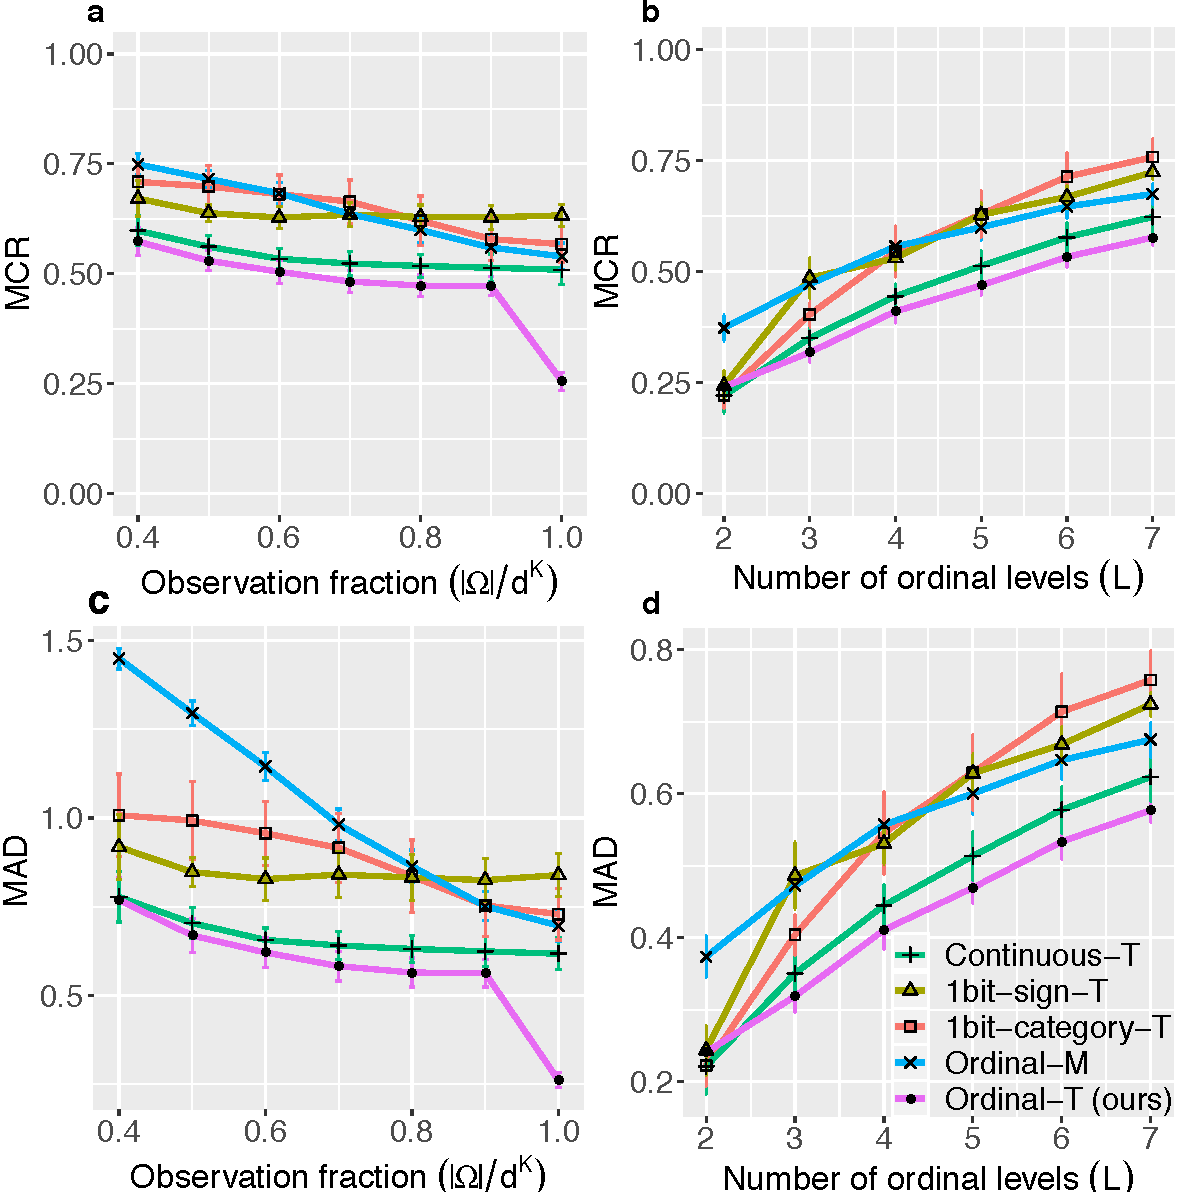
\includegraphics[width=.8\textwidth]{panel3.pdf}
  \end{center}
  \caption{Performance comparison for predicting the median label. (a,c) Prediction errors versus sample complexity $\rho=|\Omega|/d^k$ when $L=5$. (b,d) Prediction errors versus the number of ordinal levels $L$, when $\rho=0.8.$}
\end{figure}

\section{Additional results on HCP analysis}
\subsection{Clustering based on Tucker representation}\label{sec:clustering}
We perform clustering analyses based on the Tucker representation of the estimated tensor parameter $\hat\Theta$. The procedure is motivated from the higher-order extension of Principal Component Analysis (PCA) or Singular Value Decomposition (SVD). Recall that, in the matrix case, we usually perform clustering on an $m\times n$ (normalized) matrix $X$ based on the following procedure. First, we factorize $X$ into
\begin{equation}
X = U\Sigma V^T,
\end{equation}
where $\Sigma$ is a diagonal matrix and $ U,V$ are factor matrices with orthogonal columns. Second, we take each column of $V$ as a principal axis and each row in $U\Sigma$ as principal component. A subsequent multivariate clustering method (such as $K$-means) is then applied to the $m$ rows of $U\Sigma$. 


We apply a similar clustering procedure to the estimated parameter tensor $\hat\Theta$. Based on Tucker representation of $\hat \Theta$, we have
\begin{equation}\label{eq:Tuckerest}
\hat \Theta = \hat \tC\times_1\hat \mM_1\times_2\cdots\times_K\hat \mM_K,
\end{equation}
where $\hat \tC\in\mathbb{R}^{r_1\times \cdots \times r_K}$ is the estimated core tensor, $\hat \mM_k\in\mathbb{R}^{d_k\times r_k}$ are estimated factor matrices with orthogonal columns, and $\times_k$ denotes the tensor-by-matrix multiplication~\citep{kolda2009tensor}. The mode-$k$ matricization of~\eqref{eq:Tuckerest} gives
\begin{equation}
\hat \Theta_{(k)} = \hat \mM_k\hat \tC_{(k)}\left(\hat \mM_K\otimes\cdots\otimes\hat \mM_1\right),
\end{equation}
where $\hat \Theta_{(k)} , \hat \tC_{(k)}$ denote the mode-$k$ unfolding of $\hat \Theta$ and $\hat \tC$, respectively. Then, the mode-$k$ clustering can be performed as follows. First, we take colums in $\left(\hat \mM_K\otimes\cdots\otimes\hat \mM_1\right)$ as principal axes and rows in $\hat \mM_k\hat \tC_{(k)}$ as principal components. Then, we perform $K$-means clustering method to the $d_k$ rows of the matrix $\hat \mM_k\hat \tC_{(k)}$. 

\subsection{Clustering results on HCP}
We perform clustering analysis on the 68 brain nodes using the the produce described in Section~\ref{sec:clustering}. Recall that our ordinal tensor method outputs the estimated parameter tensor $\hat\Theta\in\mathbb{R}^{68\times 68\times136}$ with rank $(23,23,8)$. 
We apply $K$-means to the mode-1 principal component matrix of size $68\times 184$ ($184=23\times8$). The elbow method suggests eight clusters among the 68 nodes (see Figure~\ref{figure:elbow}). Table~\ref{table:clustering} shows the eight clusters and their compositions. 
\begin{figure}[H]
  \label{figure:elbow}
  \begin{center}
    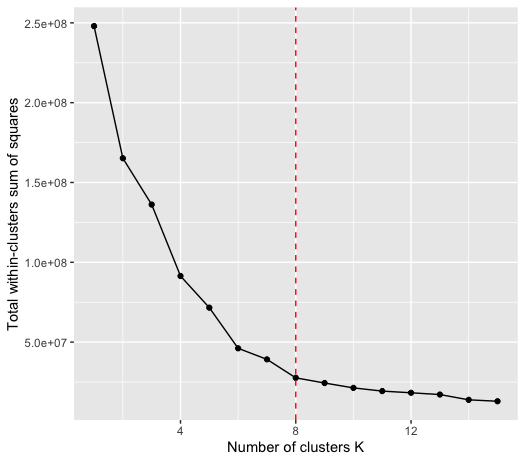
\includegraphics[width=0.48\textwidth]{elbowmethod.png}
  \end{center}
  \caption{The elbow plot for the number of clusters}
\end{figure}


We find that most brain nodes fall into cluster I and the cluster II, which can be represented as the left and right hemispheres, respectively (Figure~\ref{figure:brain image}a). From cluster III to the cluster VIII, entries within each cluster share the same name encoded in the data. For example, cluster III and cluster IV represent the {\it Supramarginal gyrus} region on the left brain and right brain. These regions are known to be in charge of interpreting tactile sensory data and involved in perception of space and limbs location~\cite{carlson2012physiology,reed1994nature}. \fixme{Miaoyan}{(I do not understand the figure and text. Why are there four panels in the Figure? Did you just plot all pairwise connections in Cluster I? Please change the edge weights using averaged connection strengths. Step 1. take average of connections over individuals. 2. plot the averaged strength between nodes within a same cluster. You also need to tune the sparsity level to make the figure interpretable...) (Texts need to be rewritten...) Figure~\ref{figure:brain image} displays the averaged connection within each cluster brain nodes. Each node is connected by edges within the same cluster and the groups can be paired as the right part and the left part of the brain.} 
The results demonstrate that our clustering successfully groups similar brain nodes together without knowledge of external annotation.

\begin{table}[H]
  \label{table:clustering}
  \center
  \begin{small}
    \footnotesize
  \begin{sc}
\begin{tabular}{|c|c|c|c|c|c|c|}
\hline
Cluster     & \multicolumn{3}{c|}{I}                                                  & \multicolumn{3}{c|}{II}                                      \\ \hline
Brain nodes & \multicolumn{3}{l|}{\begin{tabular}[c]{@{}l@{}} ``RMF\_L'',``'Fpole\_L",``Insula\_L",\\ ``SupF\_L",``CaudMF\_L",\\ ``parsTriangularis\_L",``parsOpercularis\_L",\\ ``preCentral\_L",``Tpole\_L",``SupT\_L",\\ ``SupT\_L",``postCentral\_L", ``SupP\_L",\\ ``IP\_L",``LO\_L",``MOF\_L",``SupF\_L",\\ ``IsthmusC\_L",``Precuneus\_L",\\ ``Cuneus\_L",``paraHippo\_L",\\ ``Lingual\_L",``SupT\_L",``LO\_L"\end{tabular}} & \multicolumn{3}{l|}{\begin{tabular}[c]{@{}l@{}}``RMF\_R",``Fpole\_R",``Insula\_R",\\ ``SupF\_R", ``CaudMF\_R",\\ ``parsTriangularis\_R" ,``parsOpercularis\_R",\\ ``preCentral\_R", ``Tpole\_R",``SupT\_R",\\ ``SupT\_R",``postCentral\_R",``SupP\_R",\\ ``IP\_R",``LO\_R",``MOF\_R", ``SupF\_R",\\ ``IsthmusC\_R",``Precuneus\_R",\\ ``Cuneus\_R",``paraHippo\_R",\\ ``Lingual\_R",``SupT\_R",``LO\_R"\end{tabular}} \\ \hline
Cluster      & III    & IV    & V   & VI  & VII & VIII
\\ \hline
Brain nodes & \begin{tabular}[c]{@{}c@{}}``SupraM\_L" \\ ``SupraM\_L" \\ ``SupraM\_L" \\ ``SupraM\_L"\end{tabular}                                      & \begin{tabular}[c]{@{}c@{}}``SupraM\_R" \\ ``SupraM\_R" \\ ``SupraM\_R" \\ ``SupraM\_R"\end{tabular}                                      & \begin{tabular}[c]{@{}c@{}}``IT\_L" \\ ``IT\_L" \\ ``IT\_L"\end{tabular}                                      & \begin{tabular}[c]{@{}c@{}}``IT\_R" \\ ``IT\_R" \\ ``IT\_R"\end{tabular}                                                          & \begin{tabular}[c]{@{}c@{}}``MT\_L" \\ ``MT\_L" \\ ``MT\_L"\end{tabular}                                                         & \begin{tabular}[c]{@{}c@{}}``MT\_R" \\ ``MT\_R"\\ ``MT\_R"\end{tabular}                                                         \\ \hline
\end{tabular}
\end{sc}
\end{small}
\caption{Clustering result of brain nodes. The last alphabet in the node name indicates the left brain (`L' ) and the right brain (`R') {\color{red} Please use node names from Github.../../BrainNetViewer\_20171031/Data/miaoyan/Desikan\_miaoyan.node.txt. Please remove the quote.} }
\end{table}

\begin{figure}[H]
  \centering
 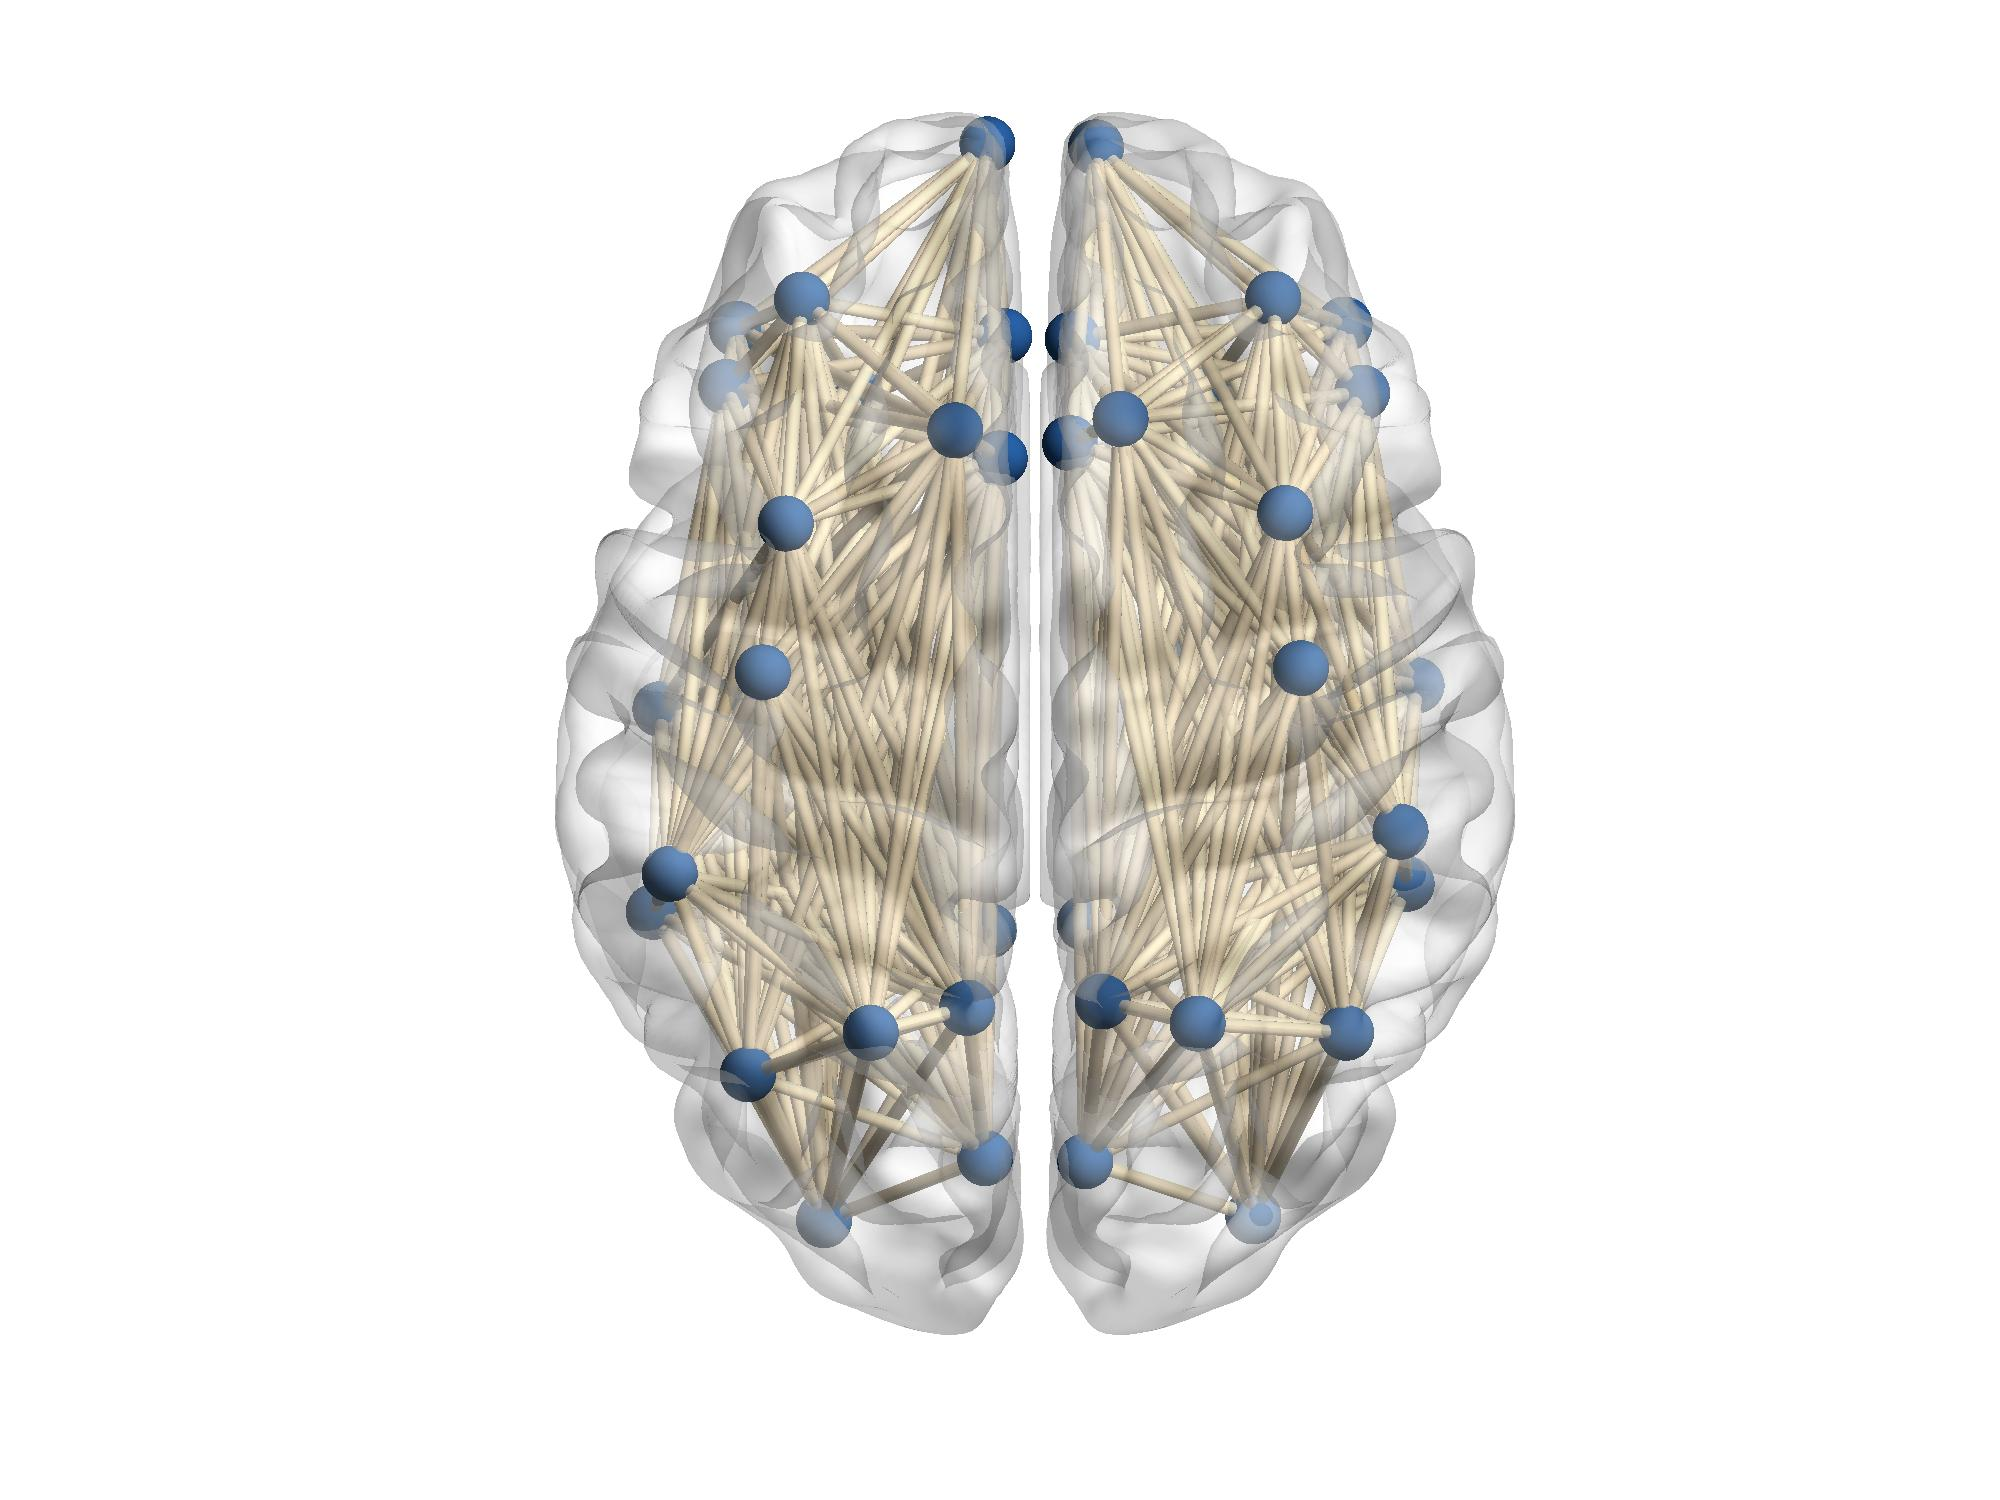
\includegraphics[width = 0.45\textwidth]{brain1.jpg}
 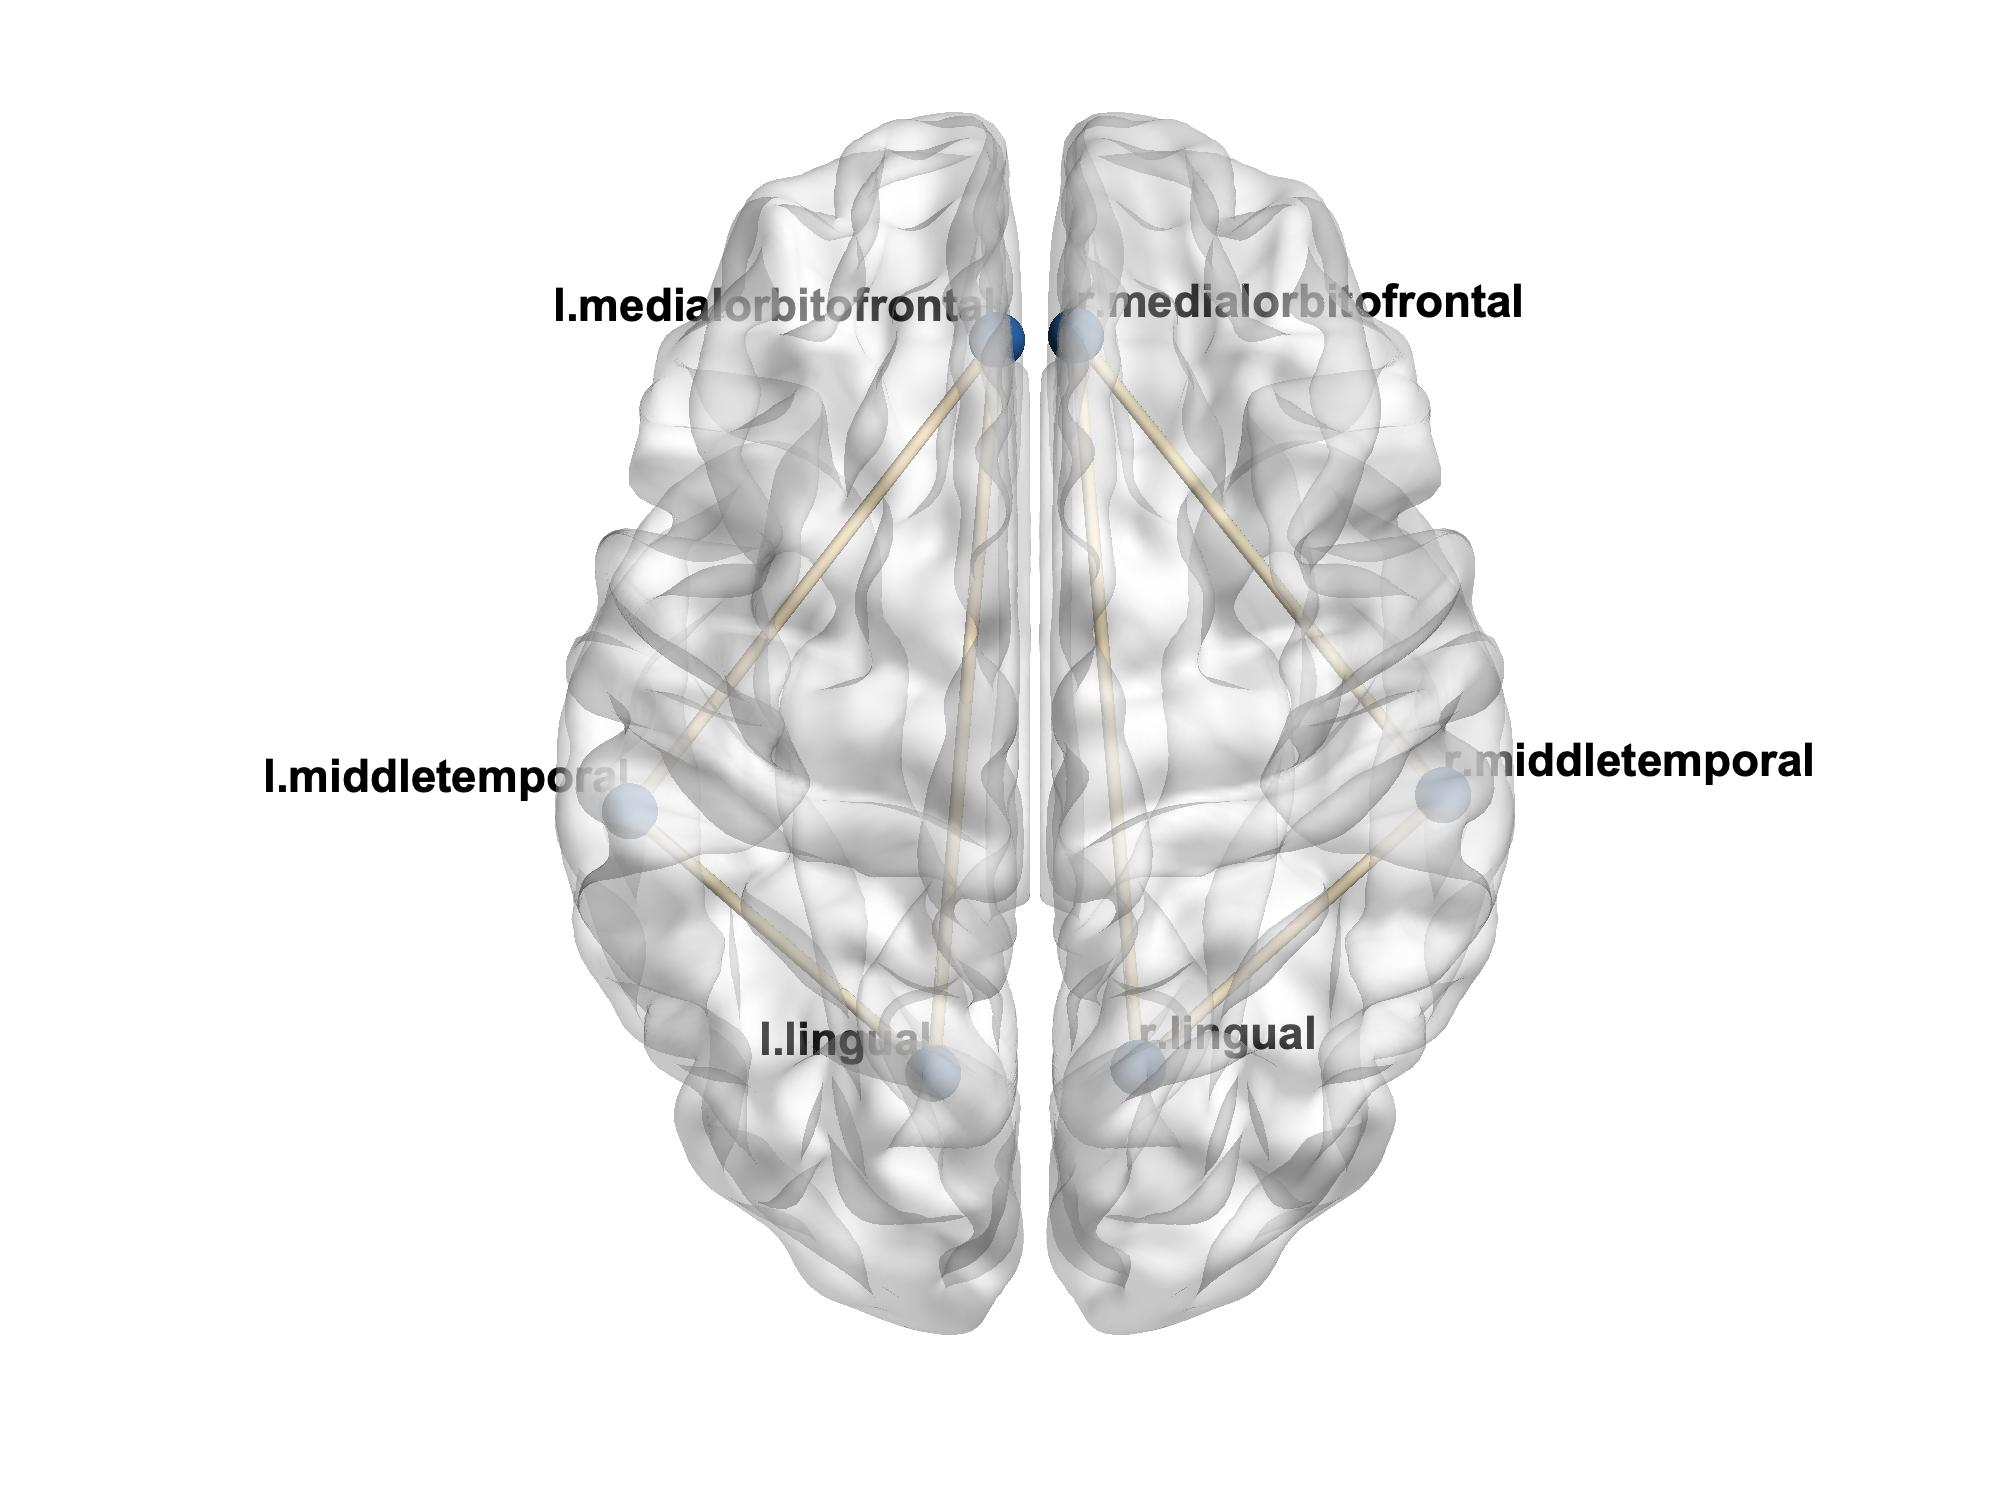
\includegraphics[width = 0.45\textwidth]{brain2.jpg}
 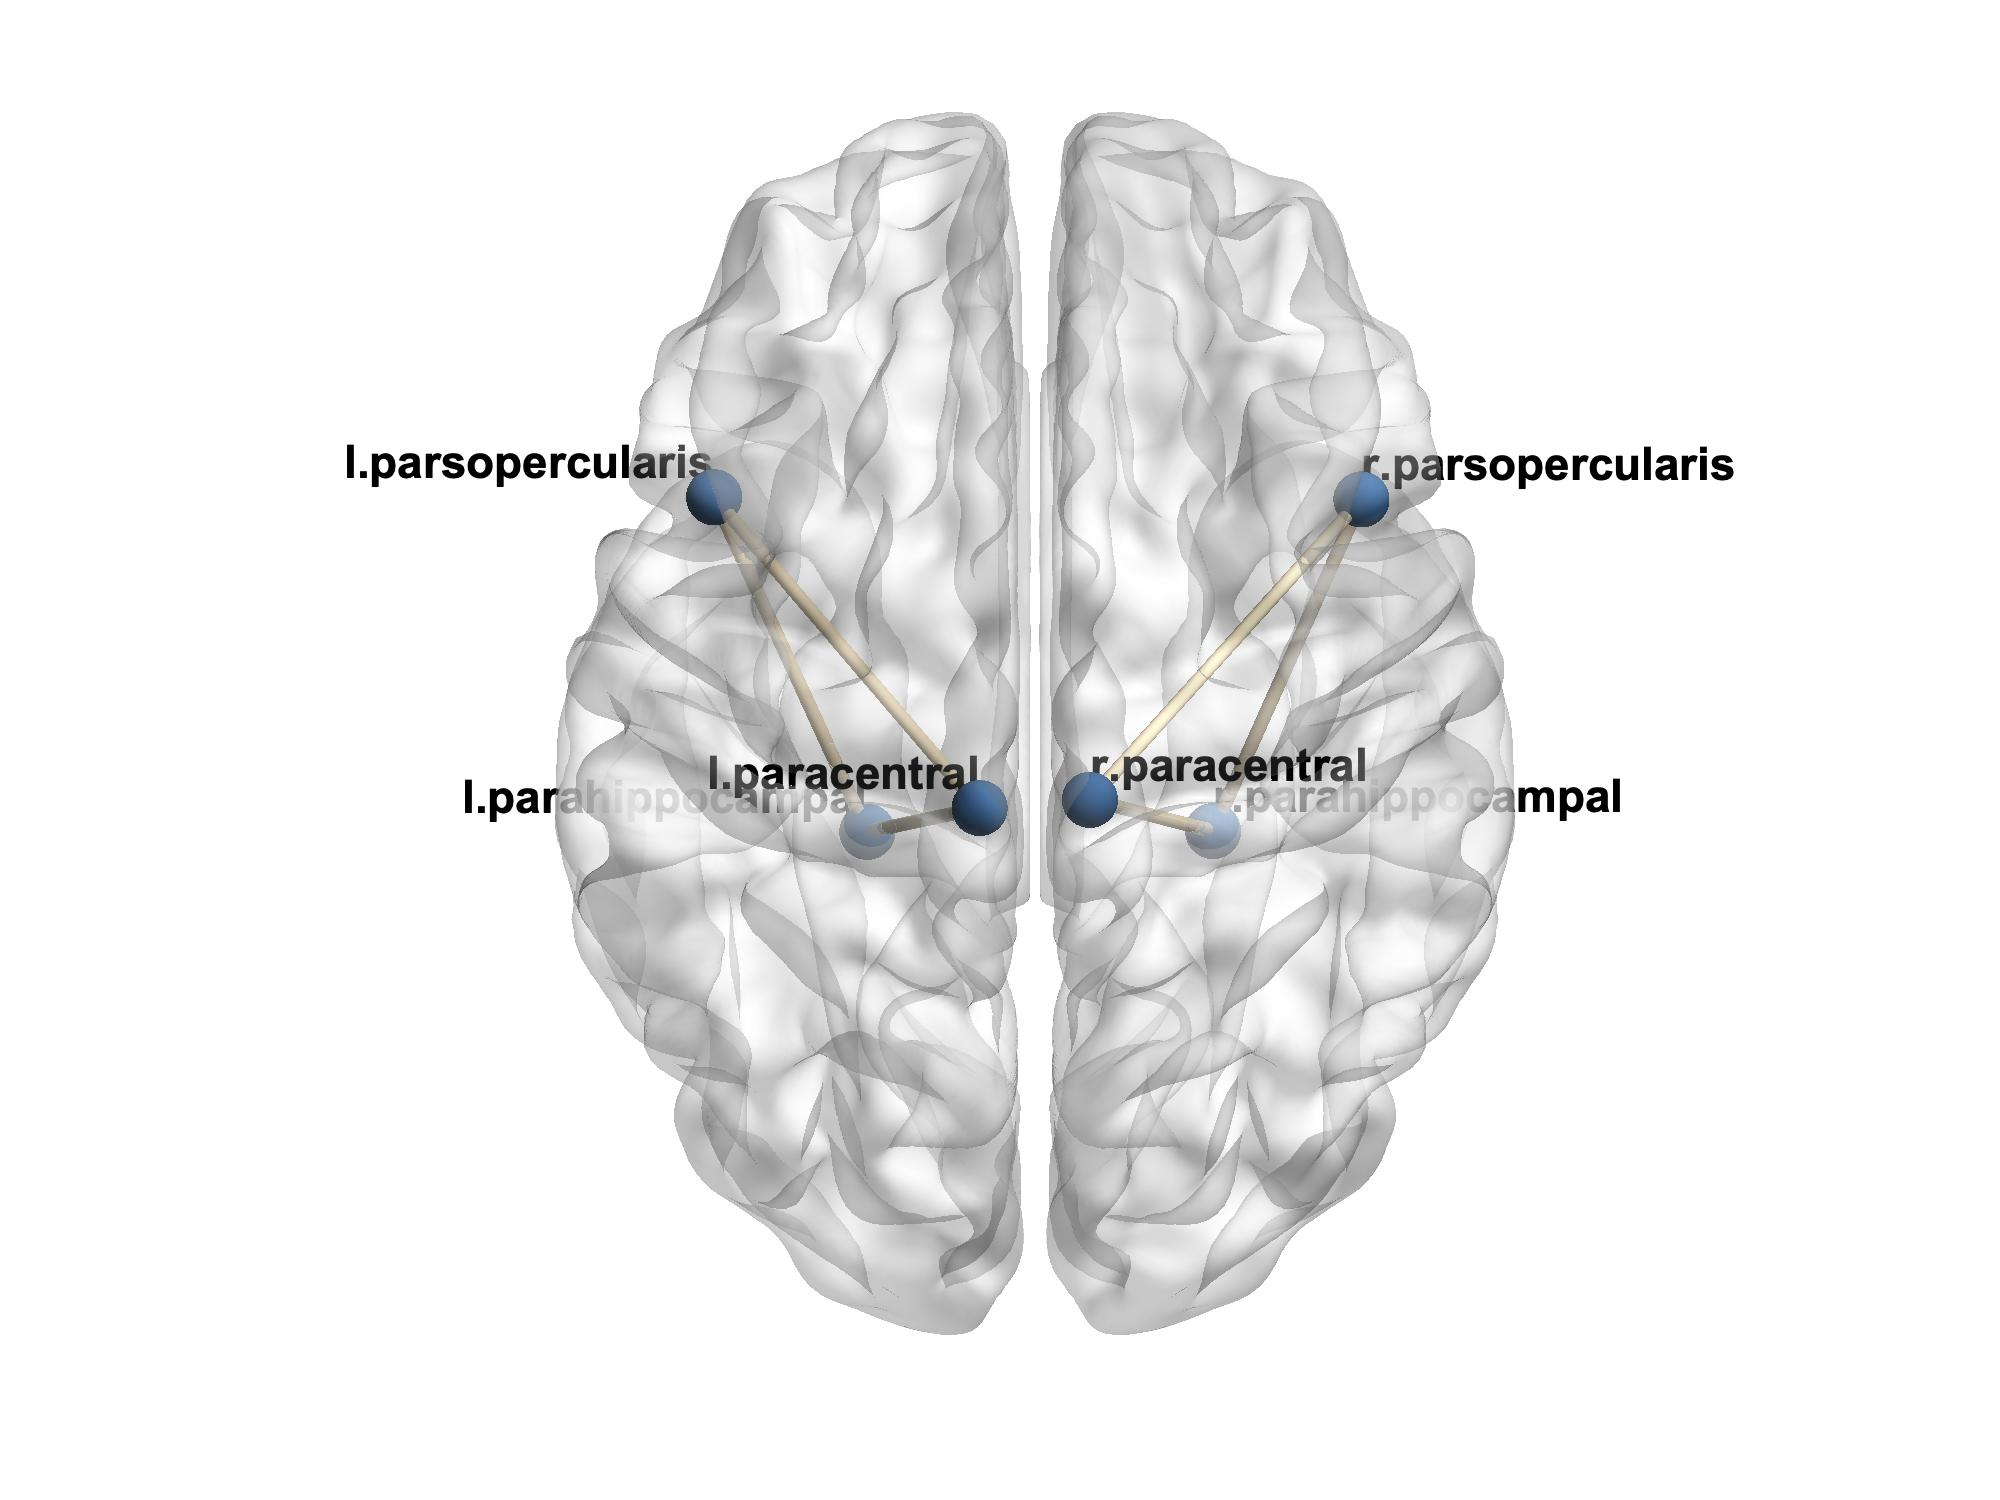
\includegraphics[width = 0.45\textwidth]{brain3.jpg}
 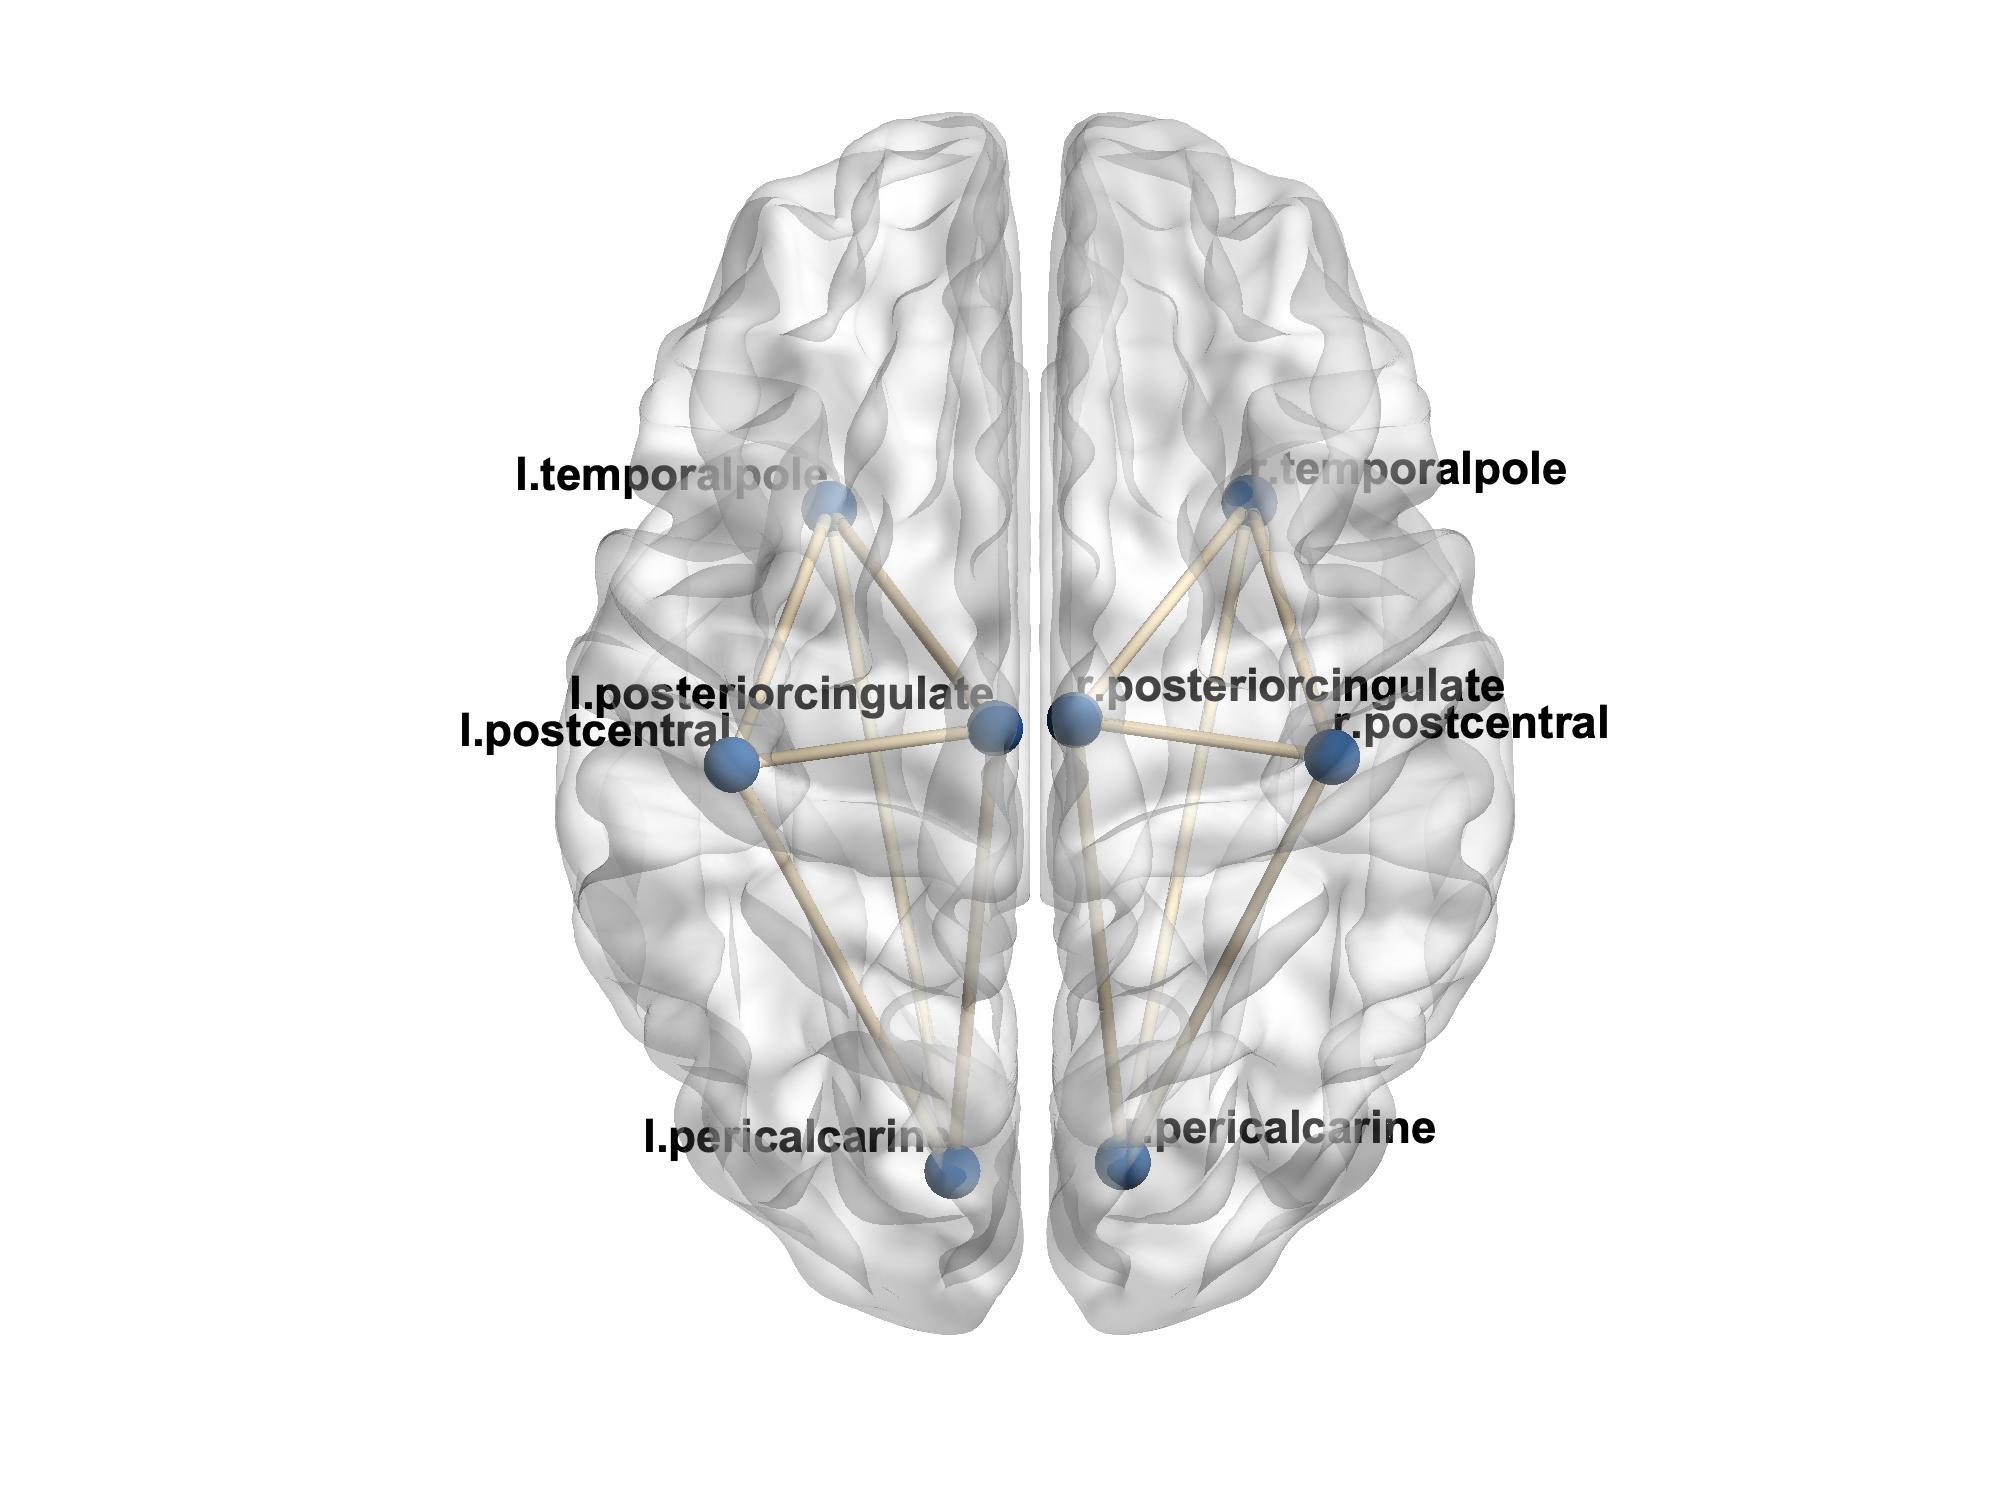
\includegraphics[width = 0.45\textwidth]{brain4.jpg}
  \label{figure:brain image}
  \caption{Averaged connection within each of the eight clusters. \fixme{Miaoyan}{Nodes within each cluster are connected by edges?}}
\end{figure}

\bibliographystyle{plainnat}
\bibliography{tensor_wang}

\end{document}
